%% Copyright 2008, The TPIE development team
%% 
%% This file is part of TPIE.
%% 
%% TPIE is free software: you can redistribute it and/or modify it under
%% the terms of the GNU Lesser General Public License as published by the
%% Free Software Foundation, either version 3 of the License, or (at your
%% option) any later version.
%% 
%% TPIE is distributed in the hope that it will be useful, but WITHOUT ANY
%% WARRANTY; without even the implied warranty of MERCHANTABILITY or
%% FITNESS FOR A PARTICULAR PURPOSE.  See the GNU Lesser General Public
%% License for more details.
%% 
%% You should have received a copy of the GNU Lesser General Public License
%% along with TPIE.  If not, see <http:%%www.gnu.org/licenses/>

\chapter{Overview}

\tobewritten (Block oriented part of TPIE)\comment{LA: Should we also
  talk a little about memory manager somewhere in this chapter?}

The\comment{LA: Rewrite/update this this section, e.g. by removing
  parallel disk stuff and include newer references/results} data sets
involved in some modern applications are too large to fit in the main
memory of even the most powerful computers and must therefore reside
on disk.  Thus communication between internal and external memory, and
not actual computation time, often becomes the bottleneck in the
computation. This is due to the huge difference in access time of fast
internal memory and slower external memory such as disks. While
typical access time of main memory is measured in nanoseconds, a
typical access time of a disk is on the order of
milliseconds~\cite{cockcroft:sun}. So roughly speaking there is a
factor of a million difference in the access time of internal and
external memory. A good example of an applications involving massive
amounts of geometric data is NASA's Earth Observation System
(EOS)~\cite{cromp,kobler:nasa}, which is expected to manipulate
petabytes (thousands of terabytes, or millions of gigabytes) of data.

The goal of theoretical work in the area of \emph{external memory (EM)
  algorithms} (also called \emph{I/O algorithms} or \emph{out-of-core
  algorithms}) is to eliminate or minimize the I/O bottleneck through
better algorithm design. In order to cope with the high cost of
accessing data, efficient EM algorithms exploit locality in their
design.  They access a large \emph{block} of $B$ contiguous data
elements at a time and perform the necessary algorithmic steps on the
elements in the block while in the high-speed memory. The speedup can
be considerable.  A second effective strategy for EM algorithms is the
use of multiple parallel disks; whenever an input/output operation is
performed, $D$ blocks are transferred in parallel between memory and
each of the $D$ disks (one block per disk).

The study of EM algorithm design was effectively started in the late
eighties by Aggarwal and Vitter~\cite{aggarwal:input} and an important
model for designing I/O algorithms called the Parallel Disk Model
(PDM) was later proposed by Vitter and Shriver~\cite{vitter:parmem1}.
The PDM proposed that a good EM algorithm should transfer data between
main memory and disk in a blocked manner, and should use all of the
available disks concurrently. An optimal EM algorithm under this model
minimizes the number of such blocked, parallel I/O operations it
performs.
 
Subsequently, I/O algorithms for the PDM (mostly with a single disk
and single processor) have been developed for many problem domains,
including computational
geometry~\cite{aapv-fibld-01,goodrich:external,arge:buffer,arge:theory,arge:gis,aamvv-empgbtag97,arge:interval,kanellakis:indexing,ramaswamy:path,subramanian:p-range,vengroff:efficient,agarwal:efficient,zhu:further,agarwal:point,arge:scalable,arge:theory,callahan:topology,franciosa:orders,grossi:cross-tree,arge:tpie},
\index{computational geometry} graph
algorithms~\cite{chiang:external,arge:buffer,kumar:improved,abello:functional,crauser:randomized,arge:obdd,feuerstein:memory,nodine:blocking,ullman:input},
\index{graph algorithms} and string
processing~\cite{ferragina:fully,ferragina:fast,arge:strings,crauser:construction}.

The use of parallel disks\index{parallel disks}
\index{disks!parallel|see{parallel disks}} has also received some
theoretical
attention~\cite{vitter:parmem1,nodine:deterministic,nodine:greed,dehne:efficient,dehne:reducing}.
There are more complicated models than the PDM, designed to address
the I/O bottleneck in different ways. These include models that
address the communication bottleneck between multiple layers in memory
hierarchies~\cite{}\comment{Add reference!}, and models incorporating
parallel processors as well as parallel
disks~\cite{cormen:challenge,dehne:efficient,dehne:reducing}.

Implementations of these theoretical results are scarce. TPIE, \emph{a
  Transparent Parallel I/O Environment}, is intended to bridge the gap
between the theory and practice of parallel I/O systems. On one hand,
TPIE attempts to provide usable implementations of (sometimes complex)
theoretical algorithms, feeding back that experience to algorithm
designers. On the other hand, TPIE also accommodates the use of
heuristics from the practice of I/O algorithms in order to achieve
maximum performance. Other EM implementation work includes
benchmarking of certain geometric I/O algorithms by
Chiang~\cite{chiang:experiments}, experiments with FFT and related
algorithms by Cormen et al.~\cite{cormen:ffts}, implementation of the
buffer tree \cite{arge:buffer} by Hutchinson
et~al.~\cite{hutchinson:early}, and the LEDA-SM system for
implementing data types by Crauser et al.\cite{mehlhorn:ledasm}.
Surveys of previous work in EM algorithm design and implementation can
be found in~\cite{arge:gisbook,arge:thesis,vitter:dimacssurvey}

%As of today, gigabyte computer systems exist on desktops, and terabyte
%systems are not unheard of.  In the not too distant future, systems
%designed to manage petabytes of information will come on-line.  The most
%important characteristic of such vast amounts of data is that they cannot
%possibly be stored in the primary memories of even the most powerful
%computers. Instead, they must be stored on secondary memory, such as
%magnetic disks, or tertiary memory, such as tapes and optical memory.
%Compared to CPUs and solid state random access memory, these devices are
%extremely slow; the difference in access time is typically 2 to 5
%orders of magnitude. Because of the low speed of secondary storage, good
%performance in the Input/Output (I/O) system that links secondary storage
%to main memory and the CPU or CPUs is critical if good performance is to be
%achieved overall. Performance can be further improved if many disks can be
%efficiently used in parallel. Unfortunately, existing I/O systems generally
%do not perform adequately~\cite{patt:computer}.

%Recently, a number of parallel I/O systems have become
%available, though in most cases they have failed to take adequate advantage
%of the insights theorists have had to offer \cite{cormen:integrate-tr}.

The objectives of the TPIE project include the following:

\begin{itemize}
\item \emph{Abstract away the details of how I/O is performed} so that
  programmers need only deal with a simple high level interface.
\item \emph{Provide a collection of I/O-optimal paradigms} for large
  scale computation that are efficient not only in theory, but also in
  practice.
\item \emph{Be flexible}, allowing programmers to specify the
  functional details of computation taking place within the supported
  paradigms.  This will allow a wide variety of algorithms to be
  implemented within the system.
\item \emph{Be portable} across a variety hardware platforms.
\item \emph{Be extensible}, so that new features can be easily added
  later.
\end{itemize}

TPIE is implemented as a set of templated classes and functions in
\CPP{}.\index{C++} It also includes a small library and a set of test
and sample applications.

\section{Hardware Platforms}
\index{hardware platforms}

TPIE
%%\comment{LA: Jan and Andy please check. AD: correct, JV: correct} 
has been tested on a variety of hardware platforms with a variety of
UNIX, Linux, MacOS X, and Windows operating systems and using several
C++ compilers.  Among others, TPIE is known to compile using the gcc
compiler versions 2.95, 3.3, 3.4 and 4.0, as well as using the MS
Visual Studio 2003 compiler (with large file support - 64bit file
offsets).


\section{Future releases}
\index{Future releases} \index{Releases!future|see{future releases}}

The current release of TPIE (\version) includes the fundamental
routines for solving fundamental {\em batched} problems such as
sorting. These routines enable the programmer to write efficient and
portable implementations of algorithms that makes use of fundamental
{\em streaming} primitives~\cite{arge:gisbook,vitter:podssurvey}.
Relative\comment{LA: Update before distribution} to versions 0.8.02a
and 0.9.01a, the current version of TPIE has been updated to improve
performance and a number of bugs have been fixed. This manual has been
updated to reflect these changes and several chapters have been
expanded in order to allow the TPIE programmer to tune the system for
best performance on a given platform. A list of the major changes can
be found on the TPIE web page at
\href{http://www.cs.duke.edu/TPIE/}{\path"http://www.cs.duke.edu/TPIE/"}.
Users of TPIE are encouraged to send bug reports, etc., to
\verb|tpie@cs.duke.edu|.

The TPIE project is work in progress and several extensions and/or
improvements to TPIE are in progress, including e.g. addition of the
distribution sweeping primitive~\cite{goodrich:external}, and addition
of several application examples (examples of applications written
using TPIE can be found in the papers listed on the TPIE home page).
This manual is also very much work in progress. In fact, the manual
does not (really) cover a recent major extension to TPIE, namely the
addition of support for random access to blocks as opposed to the
stream oriented access described in this manual. This addition
facilitate implementation of indexing structures (external data
structures). The extension is briefly described in the reference part
of the manual. A major revision of TPIE (that e.g. include several
changes to classes and functions used at user level) is currently
underway and the current manual will be updated and extended ones the
revision is done.  Users interested in obtaining/testing preliminary
versions TPIE extensions/revisions are encouraged to send a request to
\verb|tpie@cs.duke.edu|.


\chapter{Obtaining and Installing TPIE}

\comment{LA: Jan check/update this and e.g add windows stuff. Add
  something about autoconf tools?}

\section{Licensing}

TPIE is available under the terms of the GNU Lesser General Public License,
\index{license} version 3. A copy of this license
appears in Appendix~\ref{app:lgpl}.

\section{Where to get TPIE}

The latest version of TPIE, \version, is an alpha test version.  It is
available through the TPIE WWW Home Page at URL
\href{http://www.cs.duke.edu/TPIE/}{\path"http://www.cs.duke.edu/TPIE/"}.

To obtain the TPIE source distribution\index{source distribution},
follow the pointers from the home page to the distribution itself,
which consists of a gzipped tar file named
\texttt{tpie\_\version.tgz}. Your Web browser should be capable of
downloading this file to your local machine.


\section{Prerequisites}
\index{GNU software}
\plabel{sec:tut-gnu-software}

To\comment{JV: This whole subsection is obsolete and should be removed.} uncompress and unarchive the distribution, you will need either the
GNU \texttt{tar} utility, or \texttt{gzip} and a \texttt{tar} program.
(the GNU version can decompress and untar at the same time with the
'\texttt{z}' option). The GNU \texttt{make} utility is also needed.
This utility is usually located in \path"/usr/local/bin/make" (or is
called \texttt{gmake}).
% \texttt{LaTeX} and associated tools are needed to generate the
%manual, and \texttt{latex2html} is required to generate the HTML version of
%the manual.

TPIE is heavily dependent on the compiler used, mainly because of the
use of \CPP{} templates. It currently requires the GNU \CPP{}
compiler, \texttt{gcc}, version~\gxxversion~ or later (it has also
been successfully compiled with \texttt{gcc} version 2.7.2.1 on some
systems). We are currently using \texttt{gcc}, version~\gxxcurrent~
for most development work on TPIE, and we expect that TPIE will also
be compatible with future version of this compiler. TPIE has also been
successfully compiled using \texttt{egcs}, version 2.91.66.

%In general, invoking the above utilities with the single command line
%argument \texttt{--version} will indicate whether they are compatible.
Information on how to obtain and install GNU software is available at
URL \\%
\href{http://www.gnu.org/software/software.html}{\path"http://www.gnu.org/software/software.html"}.


\section{Installation}\plabel{sec:tut-installation}
\index{installation}

%Once you have obtained the TPIE source distribution file
%{\tt tpie\_\version.tgz}, you must decide where to install it.
%\texttt{/usr/local/tpie/} is a typical place.


Place \texttt{tpie\_\version.tgz} in the directory in which TPIE is to
be installed, \texttt{cd} into that directory, and execute the command

\begin{flushleft}
\texttt{tar xzf tpie\_\version.tgz}
(or \texttt{gunzip -c tpie\_\version.tgz | tar xvf -} )  
\end{flushleft}

This will produce a directory \texttt{tpie\_\version} with
subdirectories \path"include/", \path"lib/", \path"lib/src/",
\path"test/", and \path"doc/".  

You should now have
a complete TPIE system, consisting of the directories listed in Figure
\ref{fig:components}.
\begin{figure}
\begin{center}
\begin{minipage}[hb]{1.0\linewidth}
\raggedright
\centering{
\begin{tabular}{|l|p{4in}|}
\hline
Directory & Contents \\
\hline
 \path"include/"  & The TPIE header files.\index{header files}\\ 

 \path"lib/"      & The TPIE run-time library.  This is relatively
 small, as most of the TPIE system remains in the form of templated header files.\index{library} \\
 \path"lib/src/"  & The source code for the TPIE run-time
                   library. \\
 \path"test/"     & A series of test applications designed to verify
                   that TPIE is operating correctly.  This
                   directory also includes the code for the
                   sample program discussed in Chapter
                   \ref{ch:samplepgmr}.\\
 \path"bin/"      & Compiled executables from the test directory. \\
 \path"apps/"     & More advanced applications than those in the test
                    directory. Example applications are described in
                    Appendix~\ref{ch:examples}.\index{test
                    applications}\\ 
 \path"doc/"      & Written documentation for TPIE,
                   consisting of the document you are
                   reading now, in DVI and Postscript(TM)
                   formats.\index{documentation}.\\
\hline
\end{tabular}}
\caption{\plabel{fig:components} Components of the TPIE distribution.}
\end{minipage}
\end{center}
\end{figure}

\subsection{Configuration for use with gcc}

Enter the directory \texttt{tpie\_\version}.  You must now configure
TPIE for your particular system.  To do this, use the command

\begin{lstlisting}
./configure
\end{lstlisting}

\index{configuration} Certain configuration options can be specified
to the \texttt{configure} script, but usually these will not be of
interest the first time TPIE is installed.  These options are
described in Section \ref{sec:customization}.

The configuration program will take some time to examine the
parameters of your system.  Once it has done so, it will produce the
various Makefiles and configuration files required to build TPIE on
your system.  When this is done, simply invoke your version of GNU
\texttt{make}:

\begin{lstlisting}
make all
\end{lstlisting}
to build the complete TPIE system.  This will build the components of
TPIE that must be tailored to your system. This includes: the TPIE
run-time library \texttt{tpie\_\version/lib/libtpie.a}, the test and
sample programs in directory \texttt{tpie\_\version/test}, and certain
header files in \texttt{tpie\_\version/include}.  

\subsection{Configuration for use with Microsoft Visual Studio .NET
  2003}

The TPIE directory contains a subdirectory named
\texttt{MSVC60}\comment{JV: This should be renamed, but I do not know
  how to rename files in CVS.} in which you can find a complete
``solution'' for building TPIE. To compile TPIE, simply open the
solution file \texttt{tpie.sln} and have Visual Studio build all
projects (by invoking ``build all'').

At this point, we find it helpful to briefly discuss how to add a
project to the TPIE solution, and we will provide an illustrated
walk-through that also explains which compilation parameters to set.

\paragraph{Step 1: Creating a new project}

Let us assume that the name of the project to be created is
\texttt{MyTestProject}. To add an empty project, select ``Add Project
$\rightarrow$ New Project\ldots'' from the ``File'' menu.

\begin{center}
  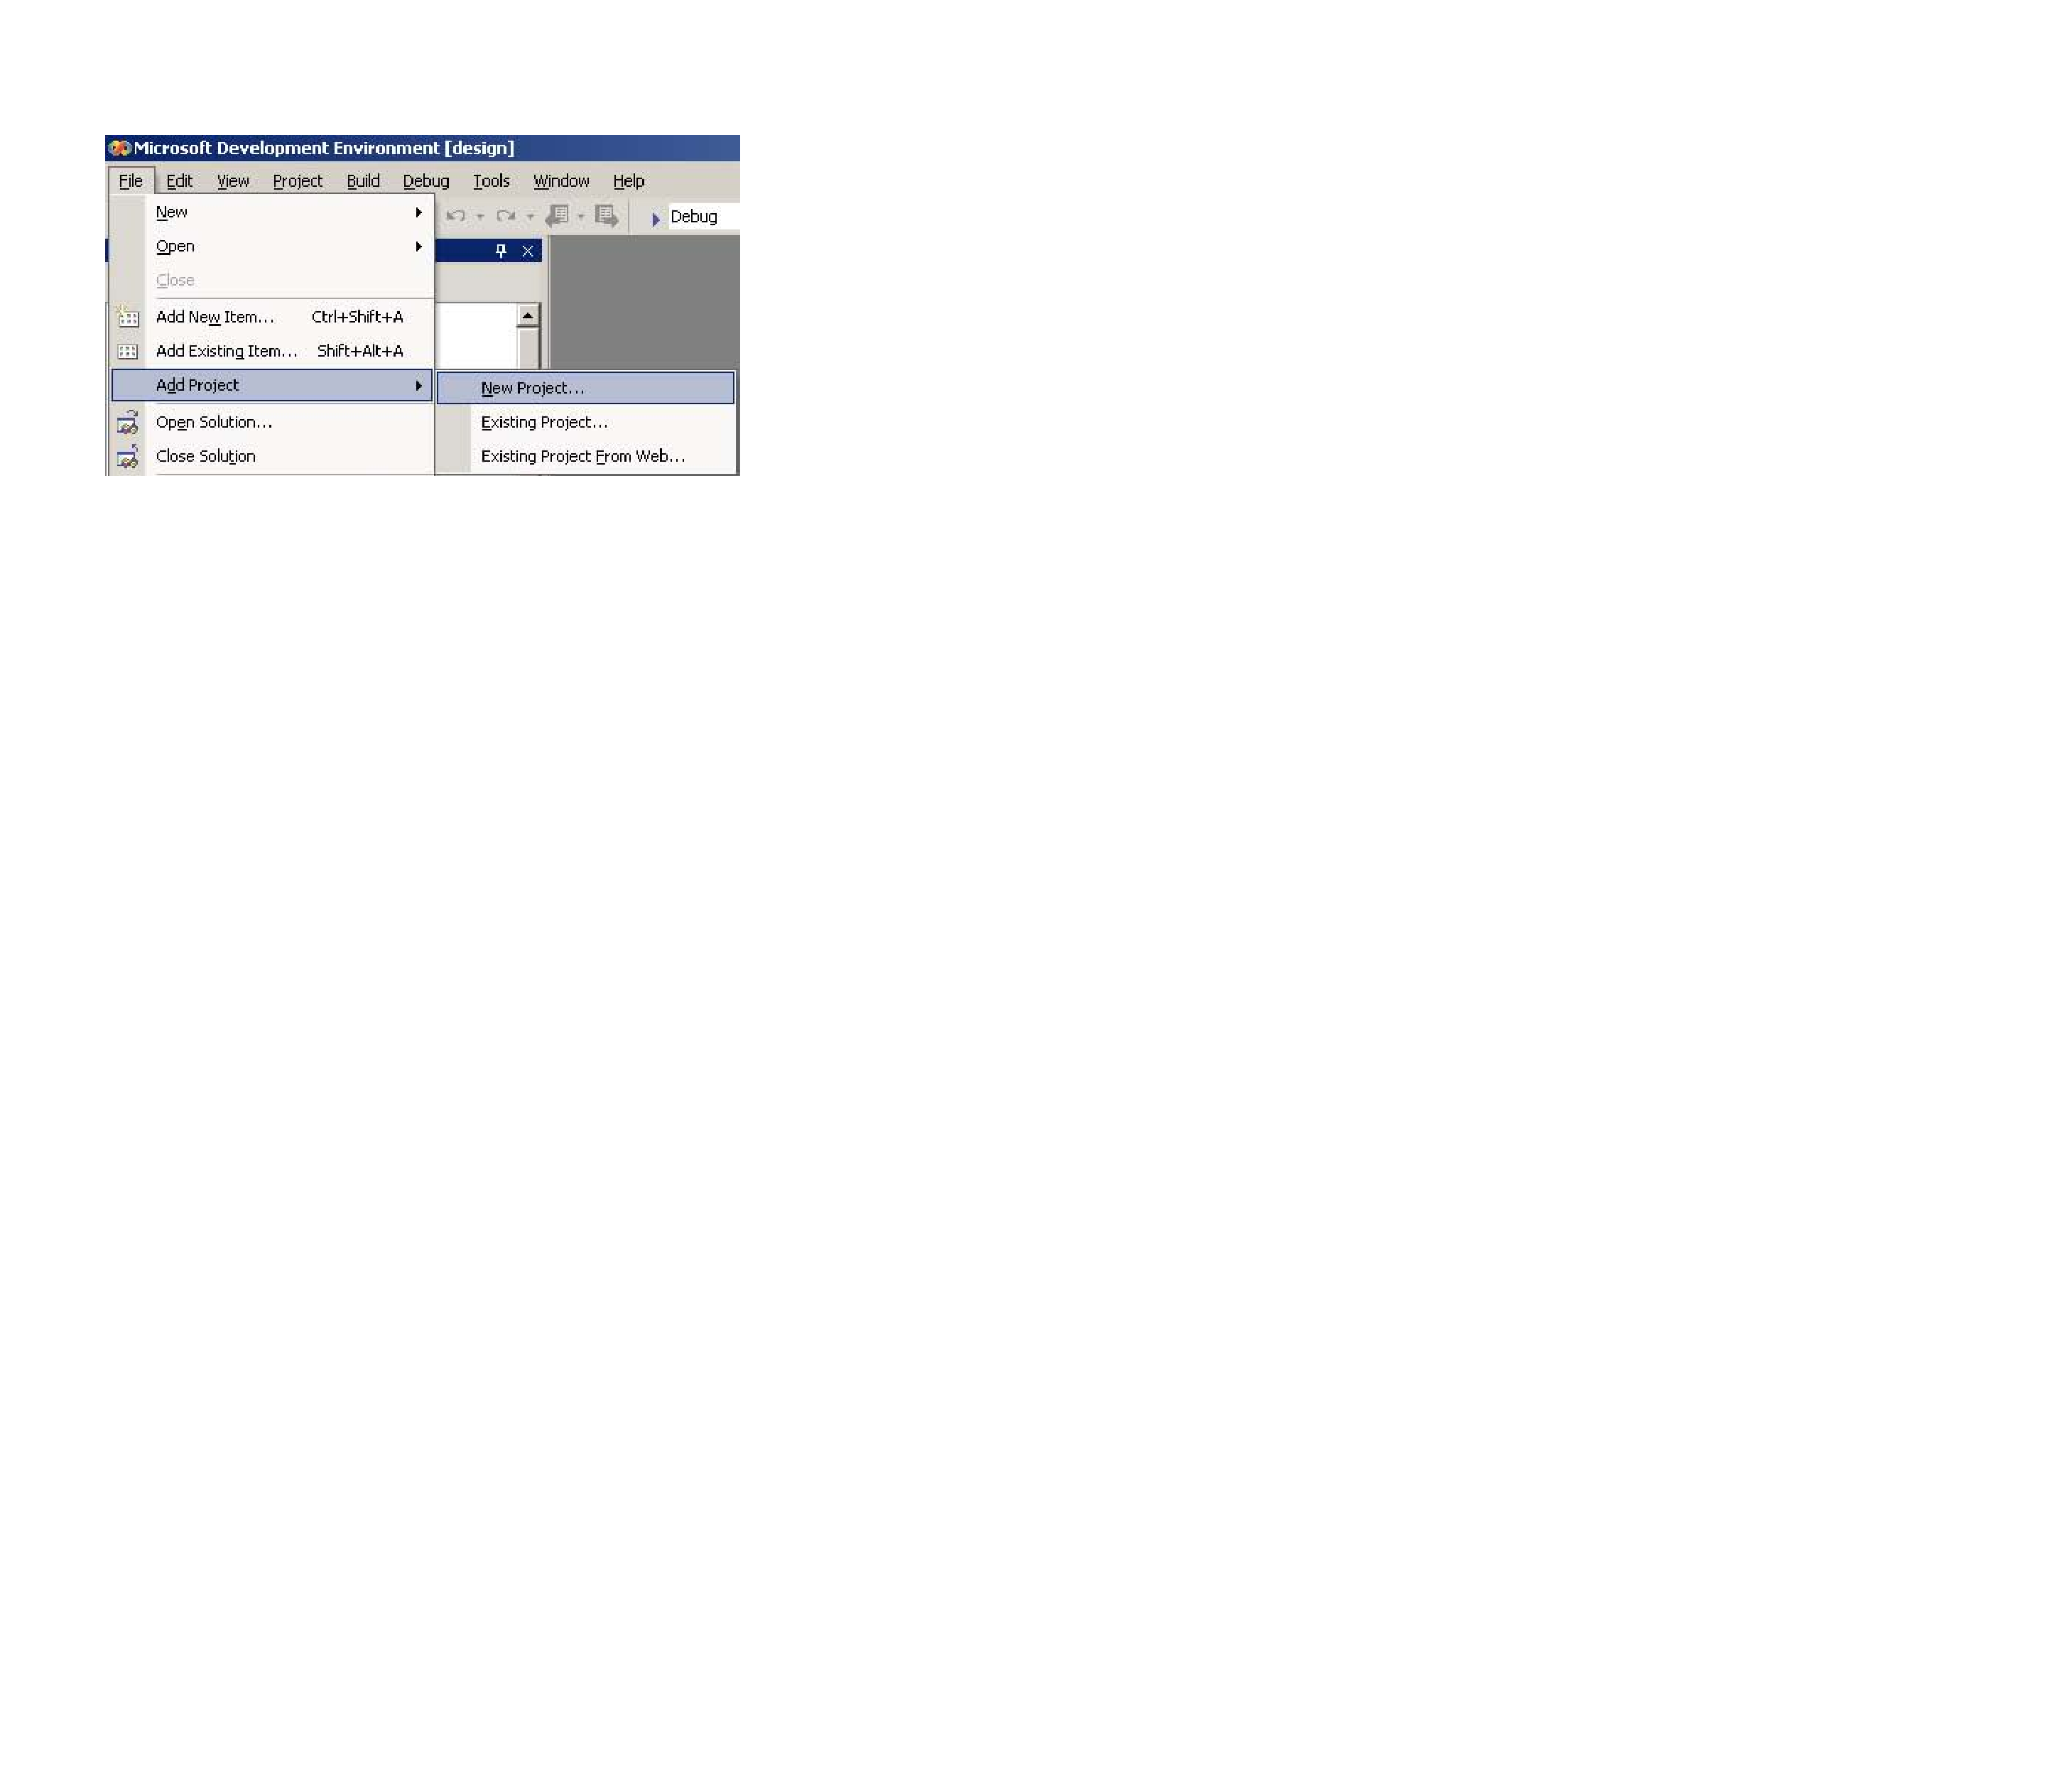
\includegraphics[scale=0.4]{figures/net_setup1.pdf}
\end{center}

Select ``Win32 Console Project'' as the type of project to be created
and enter the name (in our example \texttt{MyTestProject}) in the
dialog box. Then, click ``Ok''.

\begin{center}
  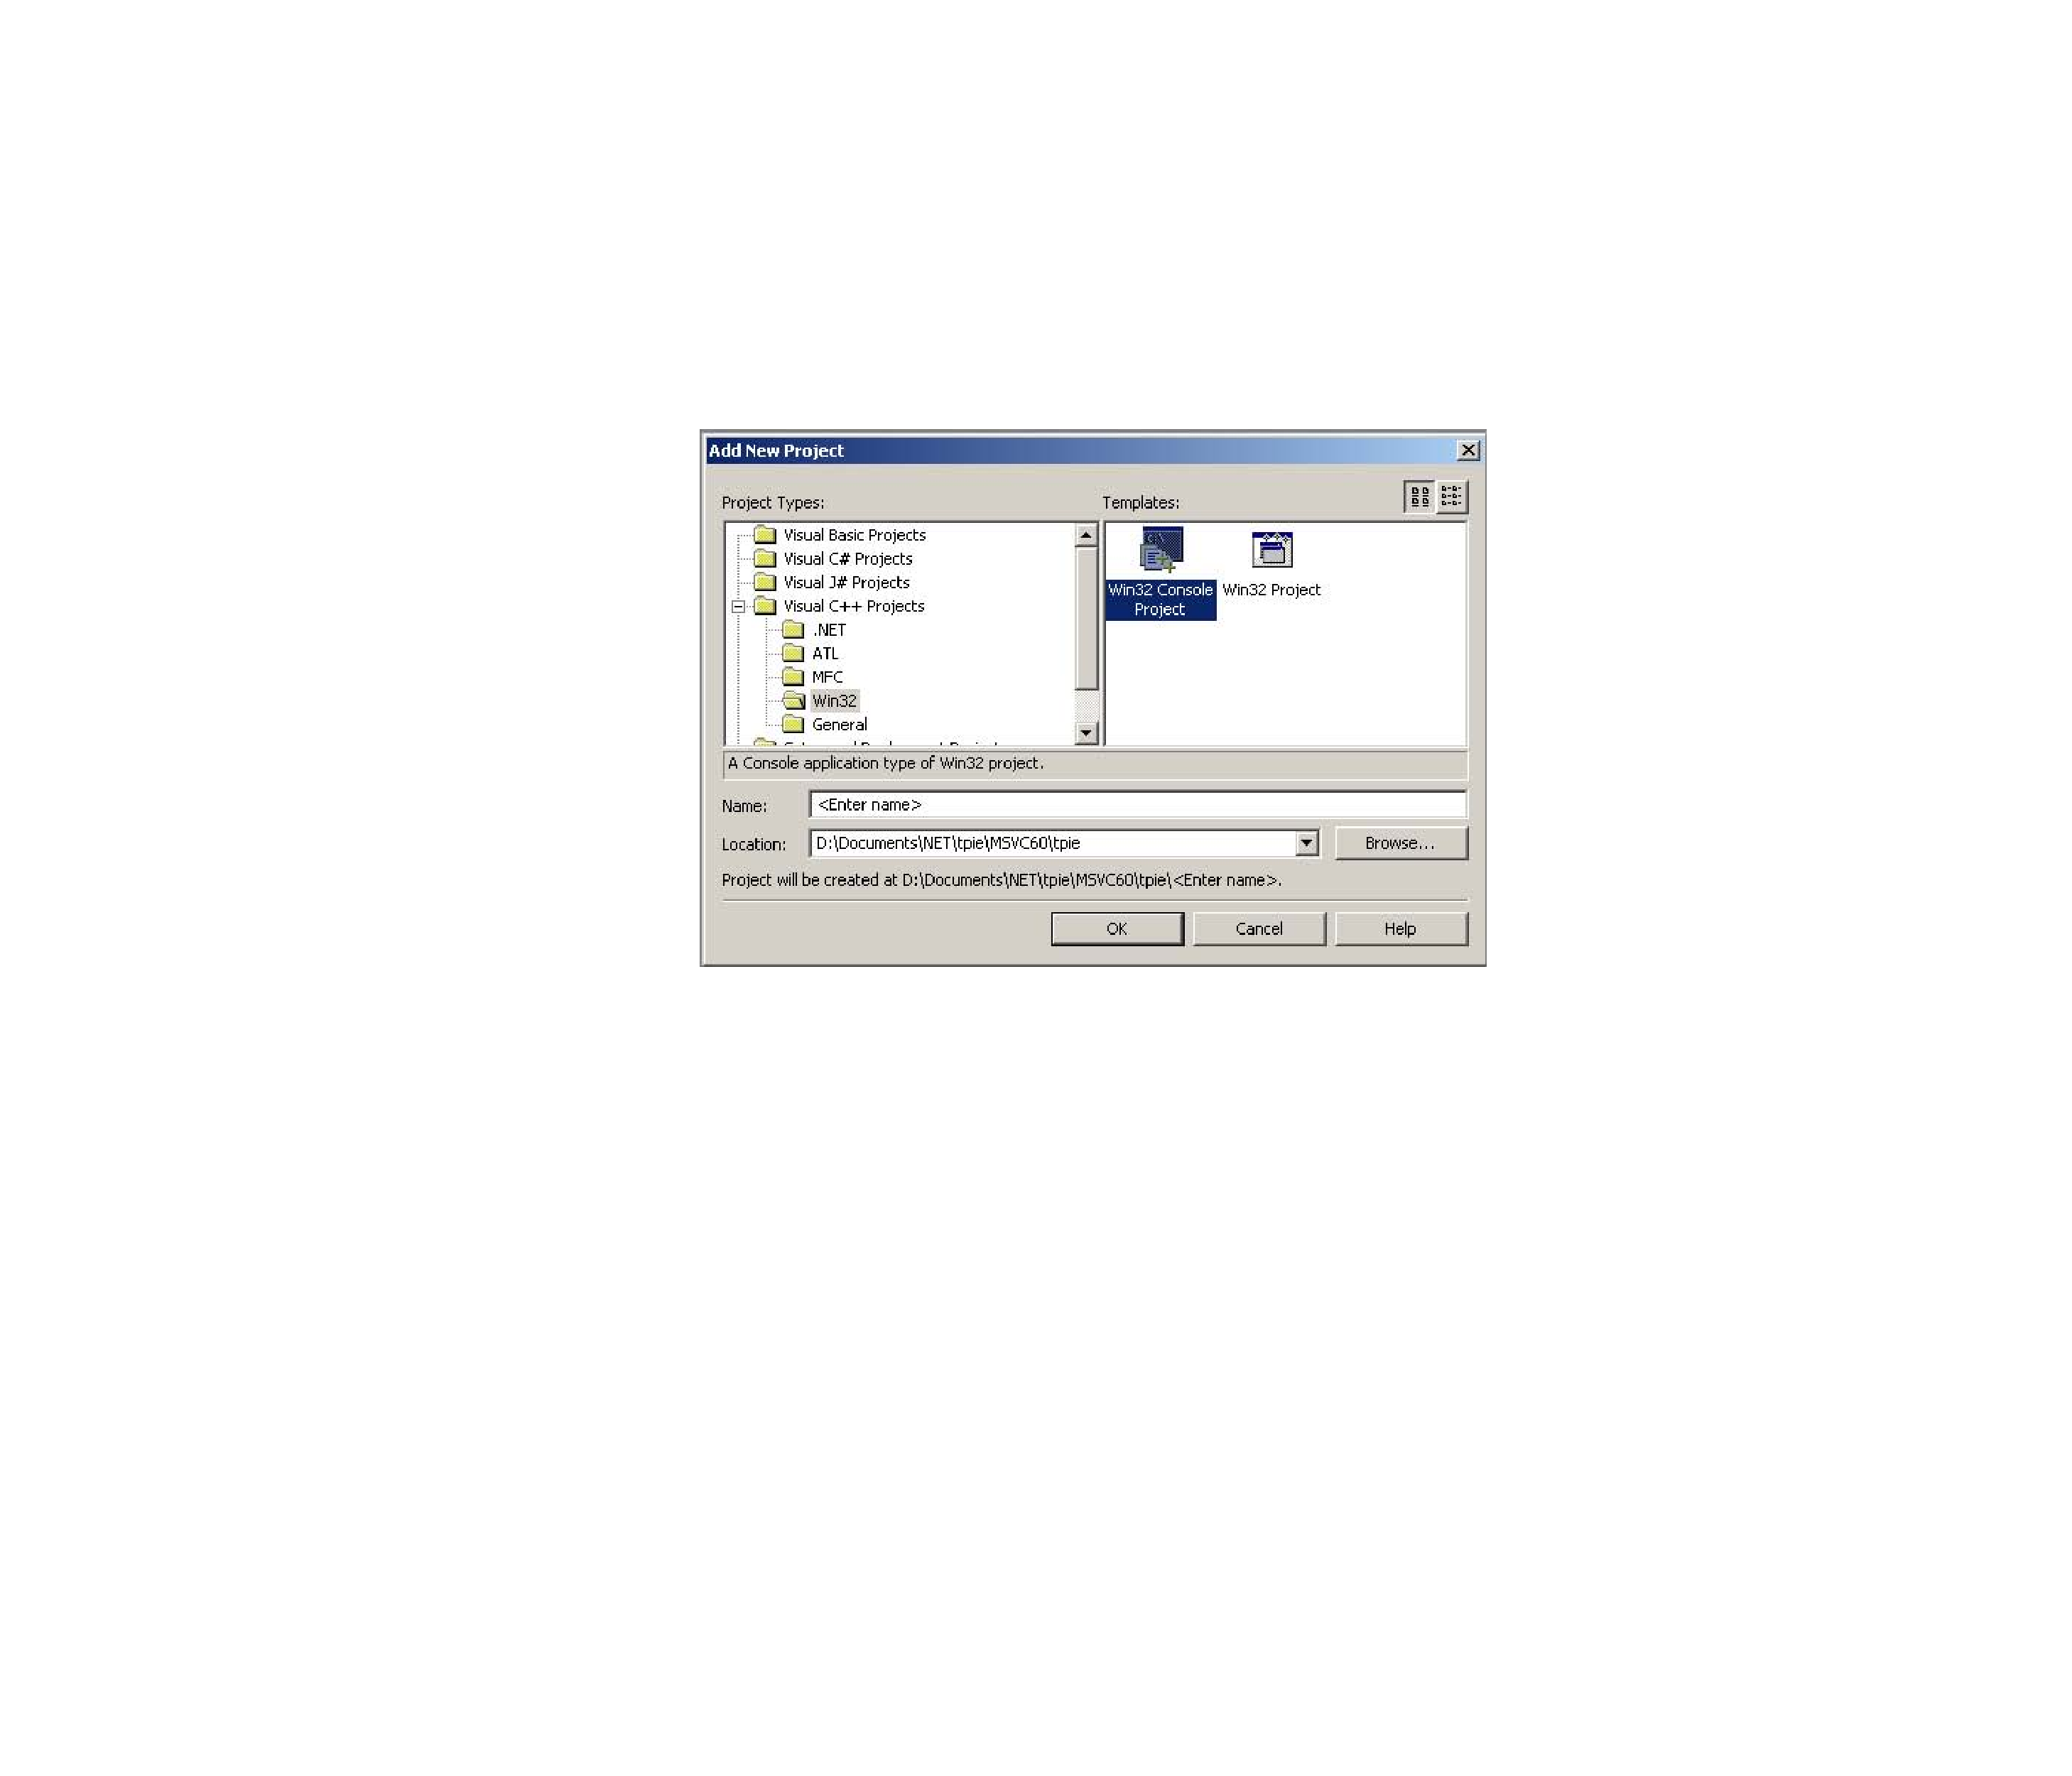
\includegraphics[scale=0.4]{figures/net_setup2.pdf}
\end{center}

To finalize creating an empty project, make sure to check the
corresponding checkbox in the next dialog. To do so, first click on
``Application Settings'', then select ``Empty project'', and confirm
by clicking the ``Finish'' button.

\begin{center}
  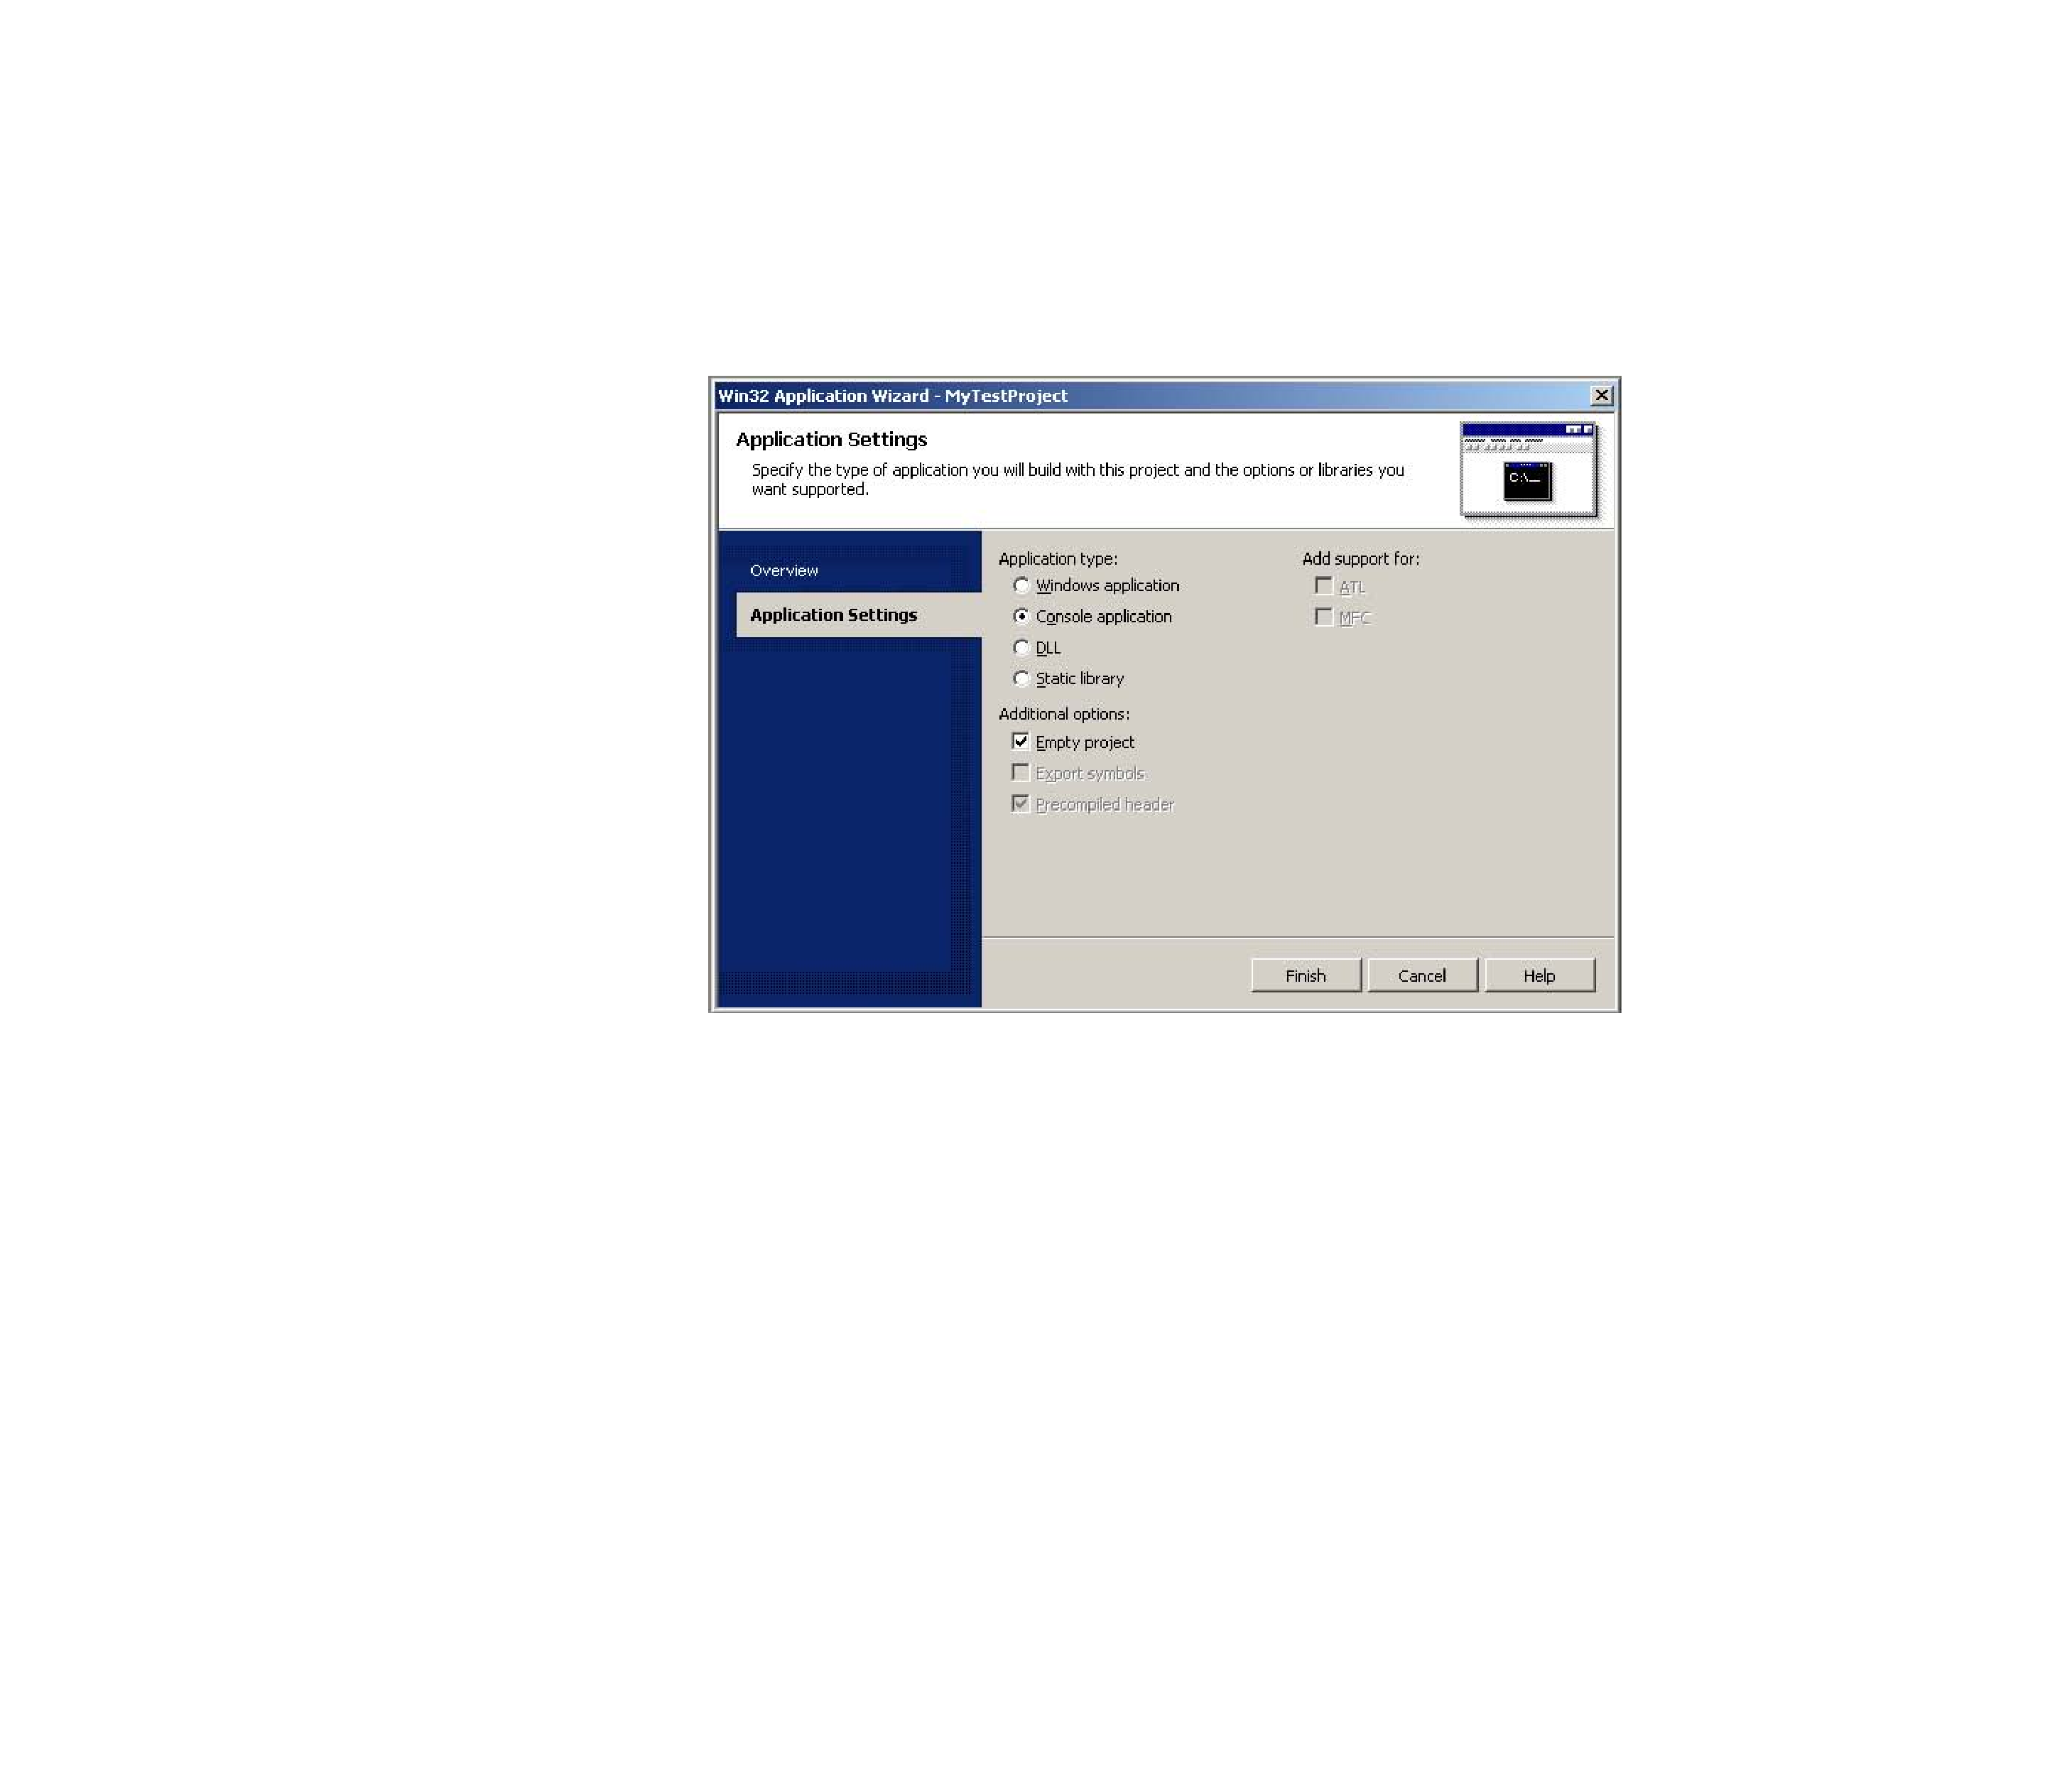
\includegraphics[scale=0.4]{figures/net_setup3.pdf}
\end{center}

A new project entry \texttt{MyTestProject} should appear in the
solution.

\paragraph{Step 2: Adding a main file}

To add an empty main file to the project, select ``Add New
Item\ldots'' from the ``File'' menu. Select the ``\texttt{C++} File''
template from the dialog and enter the file name, e.g.,
\texttt{main.cpp} in the dialog box. Confirm by clicking ``Ok''.

\begin{center}
  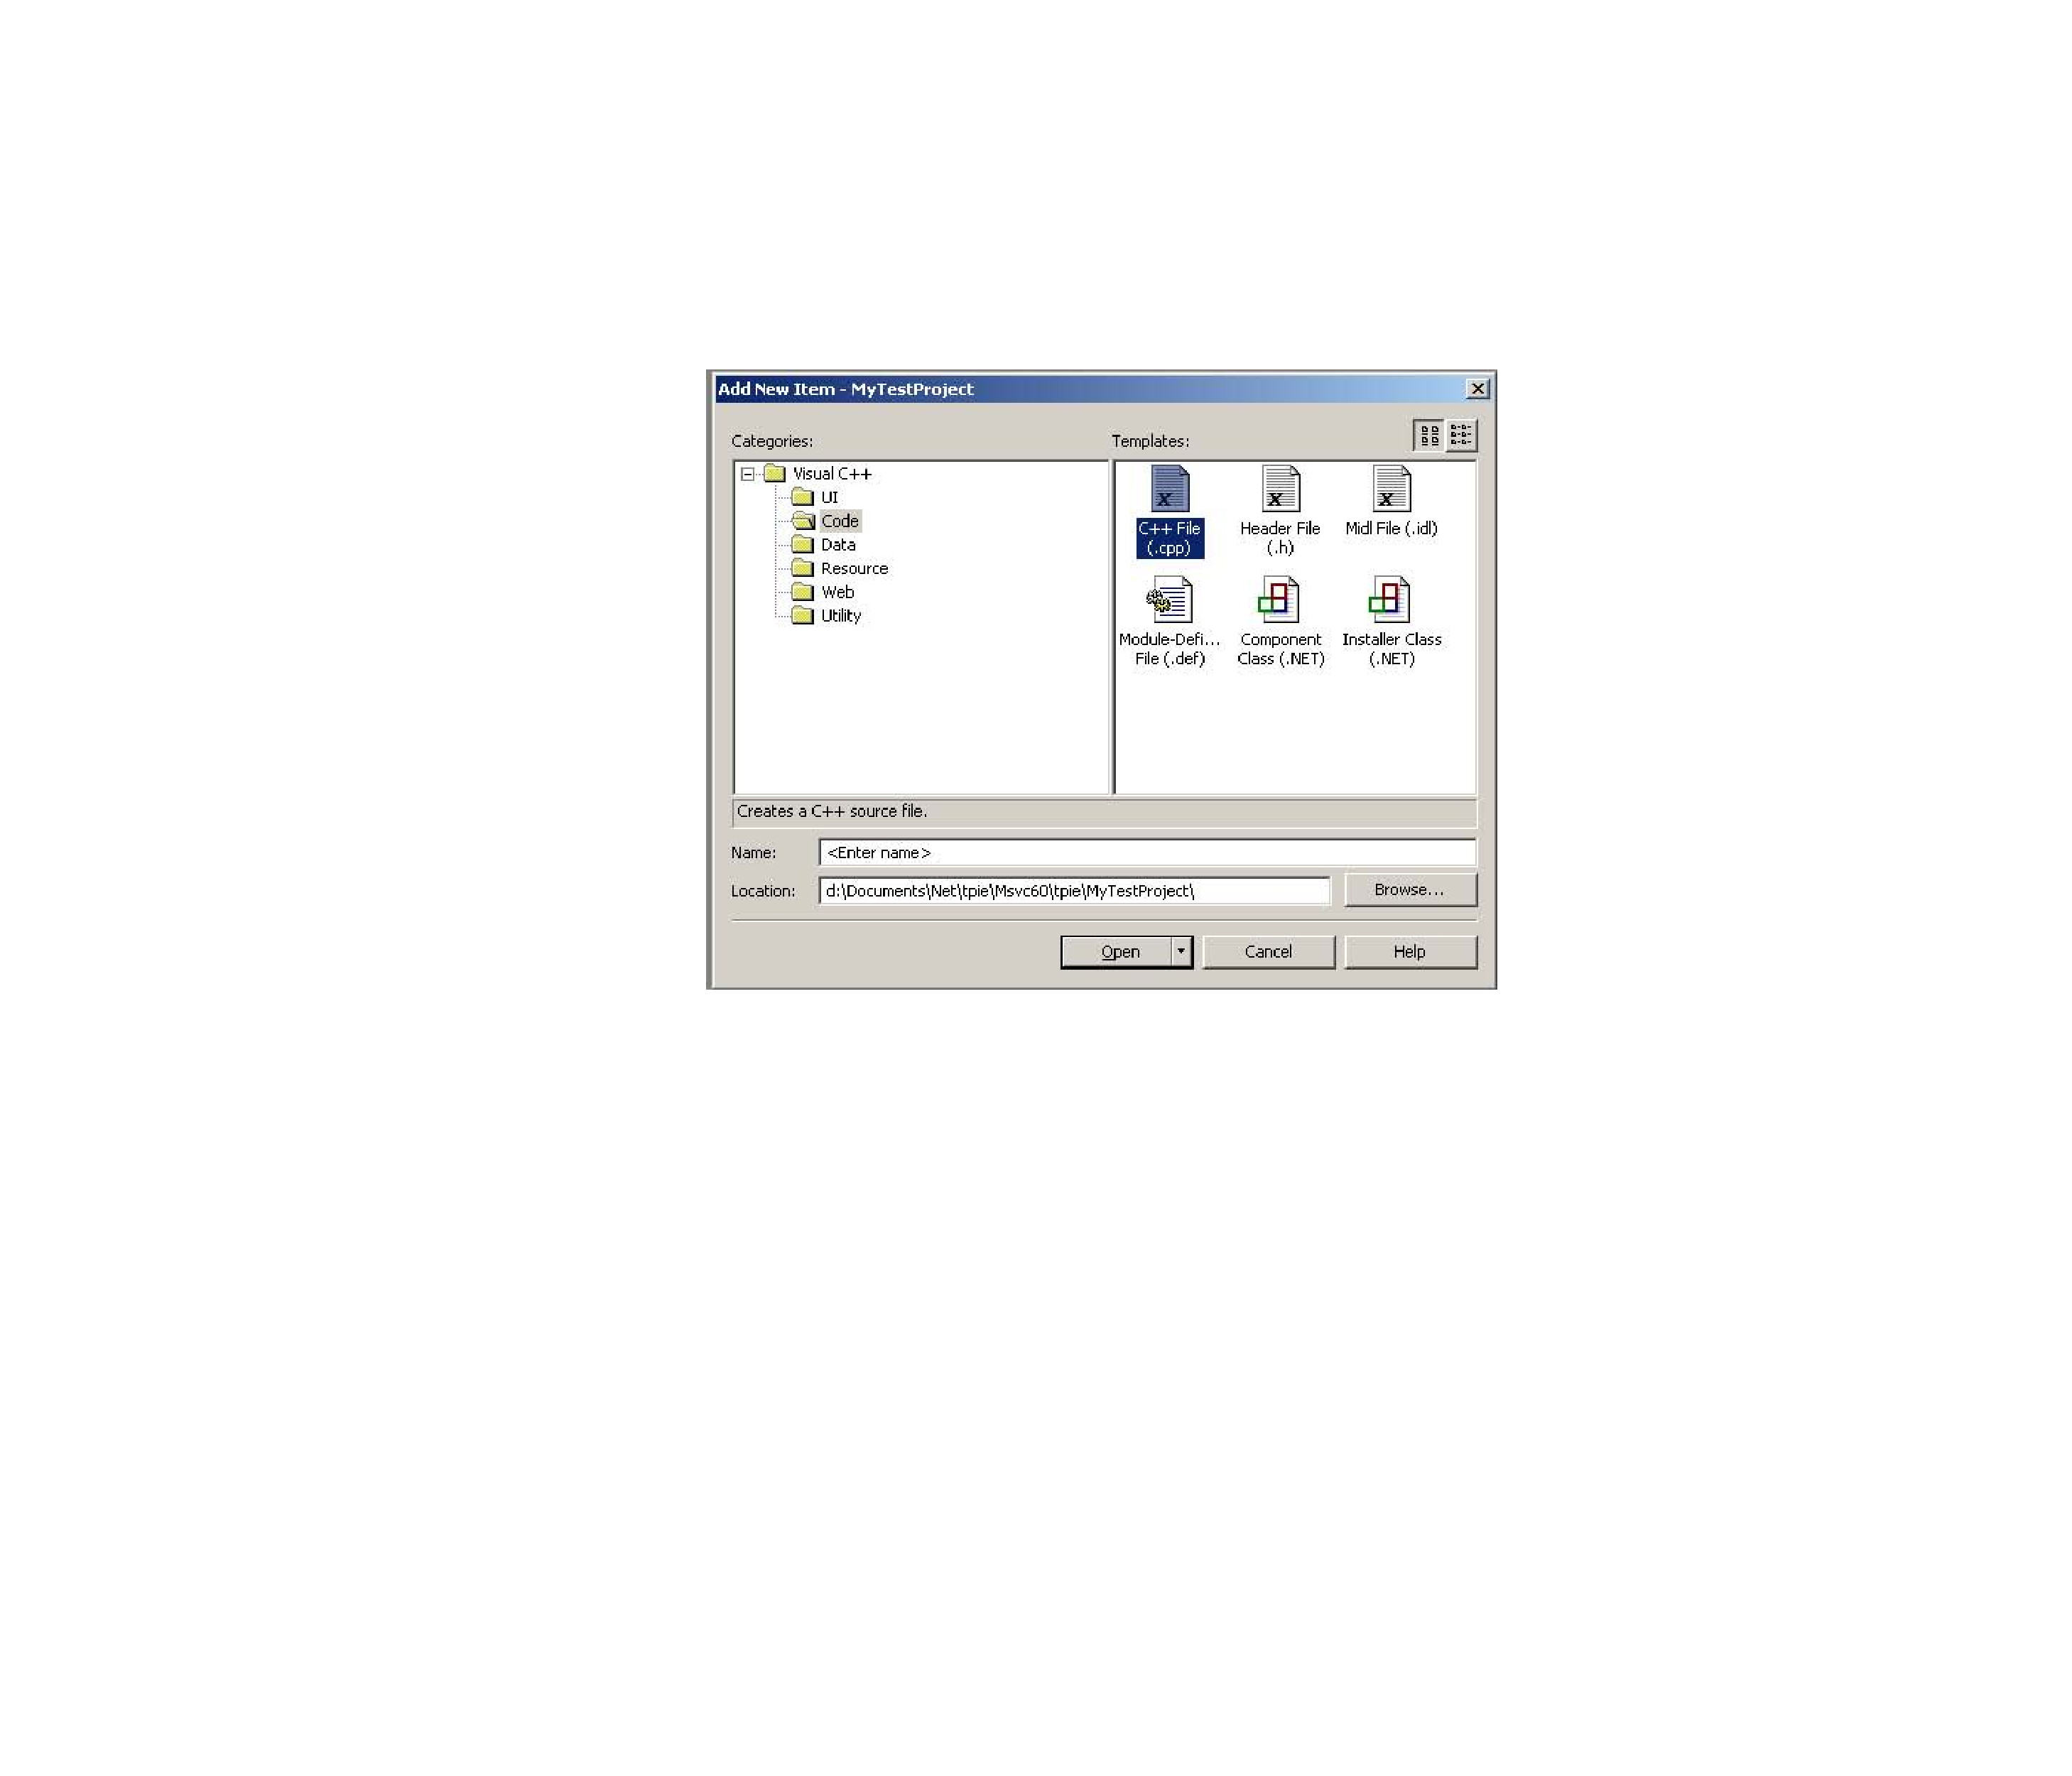
\includegraphics[scale=0.4]{figures/net_setup8.pdf}
\end{center}


\paragraph{Step 3: Setting paths and compile-time parameters}

To access the project's properties dialog, right-click on the project
entry and select the ``Properties'' entry from the pop-up menu. To
futher facilitate setting the parameters, choose the ``All
Configurations'' configuration from the upper left pulldown menu
located in the properties dialog.

The first step is to specify the include directories. Select the
``\texttt{C}/\texttt{C++}'' entry in the left column of the dialog
(note that this entry exist only if you have added a (possibly empty)
file to the project) and click on the ``General'' subentry. Enter
``\path"..\..\..\include"'' in the field ``Additional Include
Directories''. We strongly suggest to also turn on warning level 3
(compile-time switch \texttt{/W3}) and
to have the compile check for 64-bit portability issues (compile-time
switch \texttt{/Wp64}). 
 
\begin{center}
  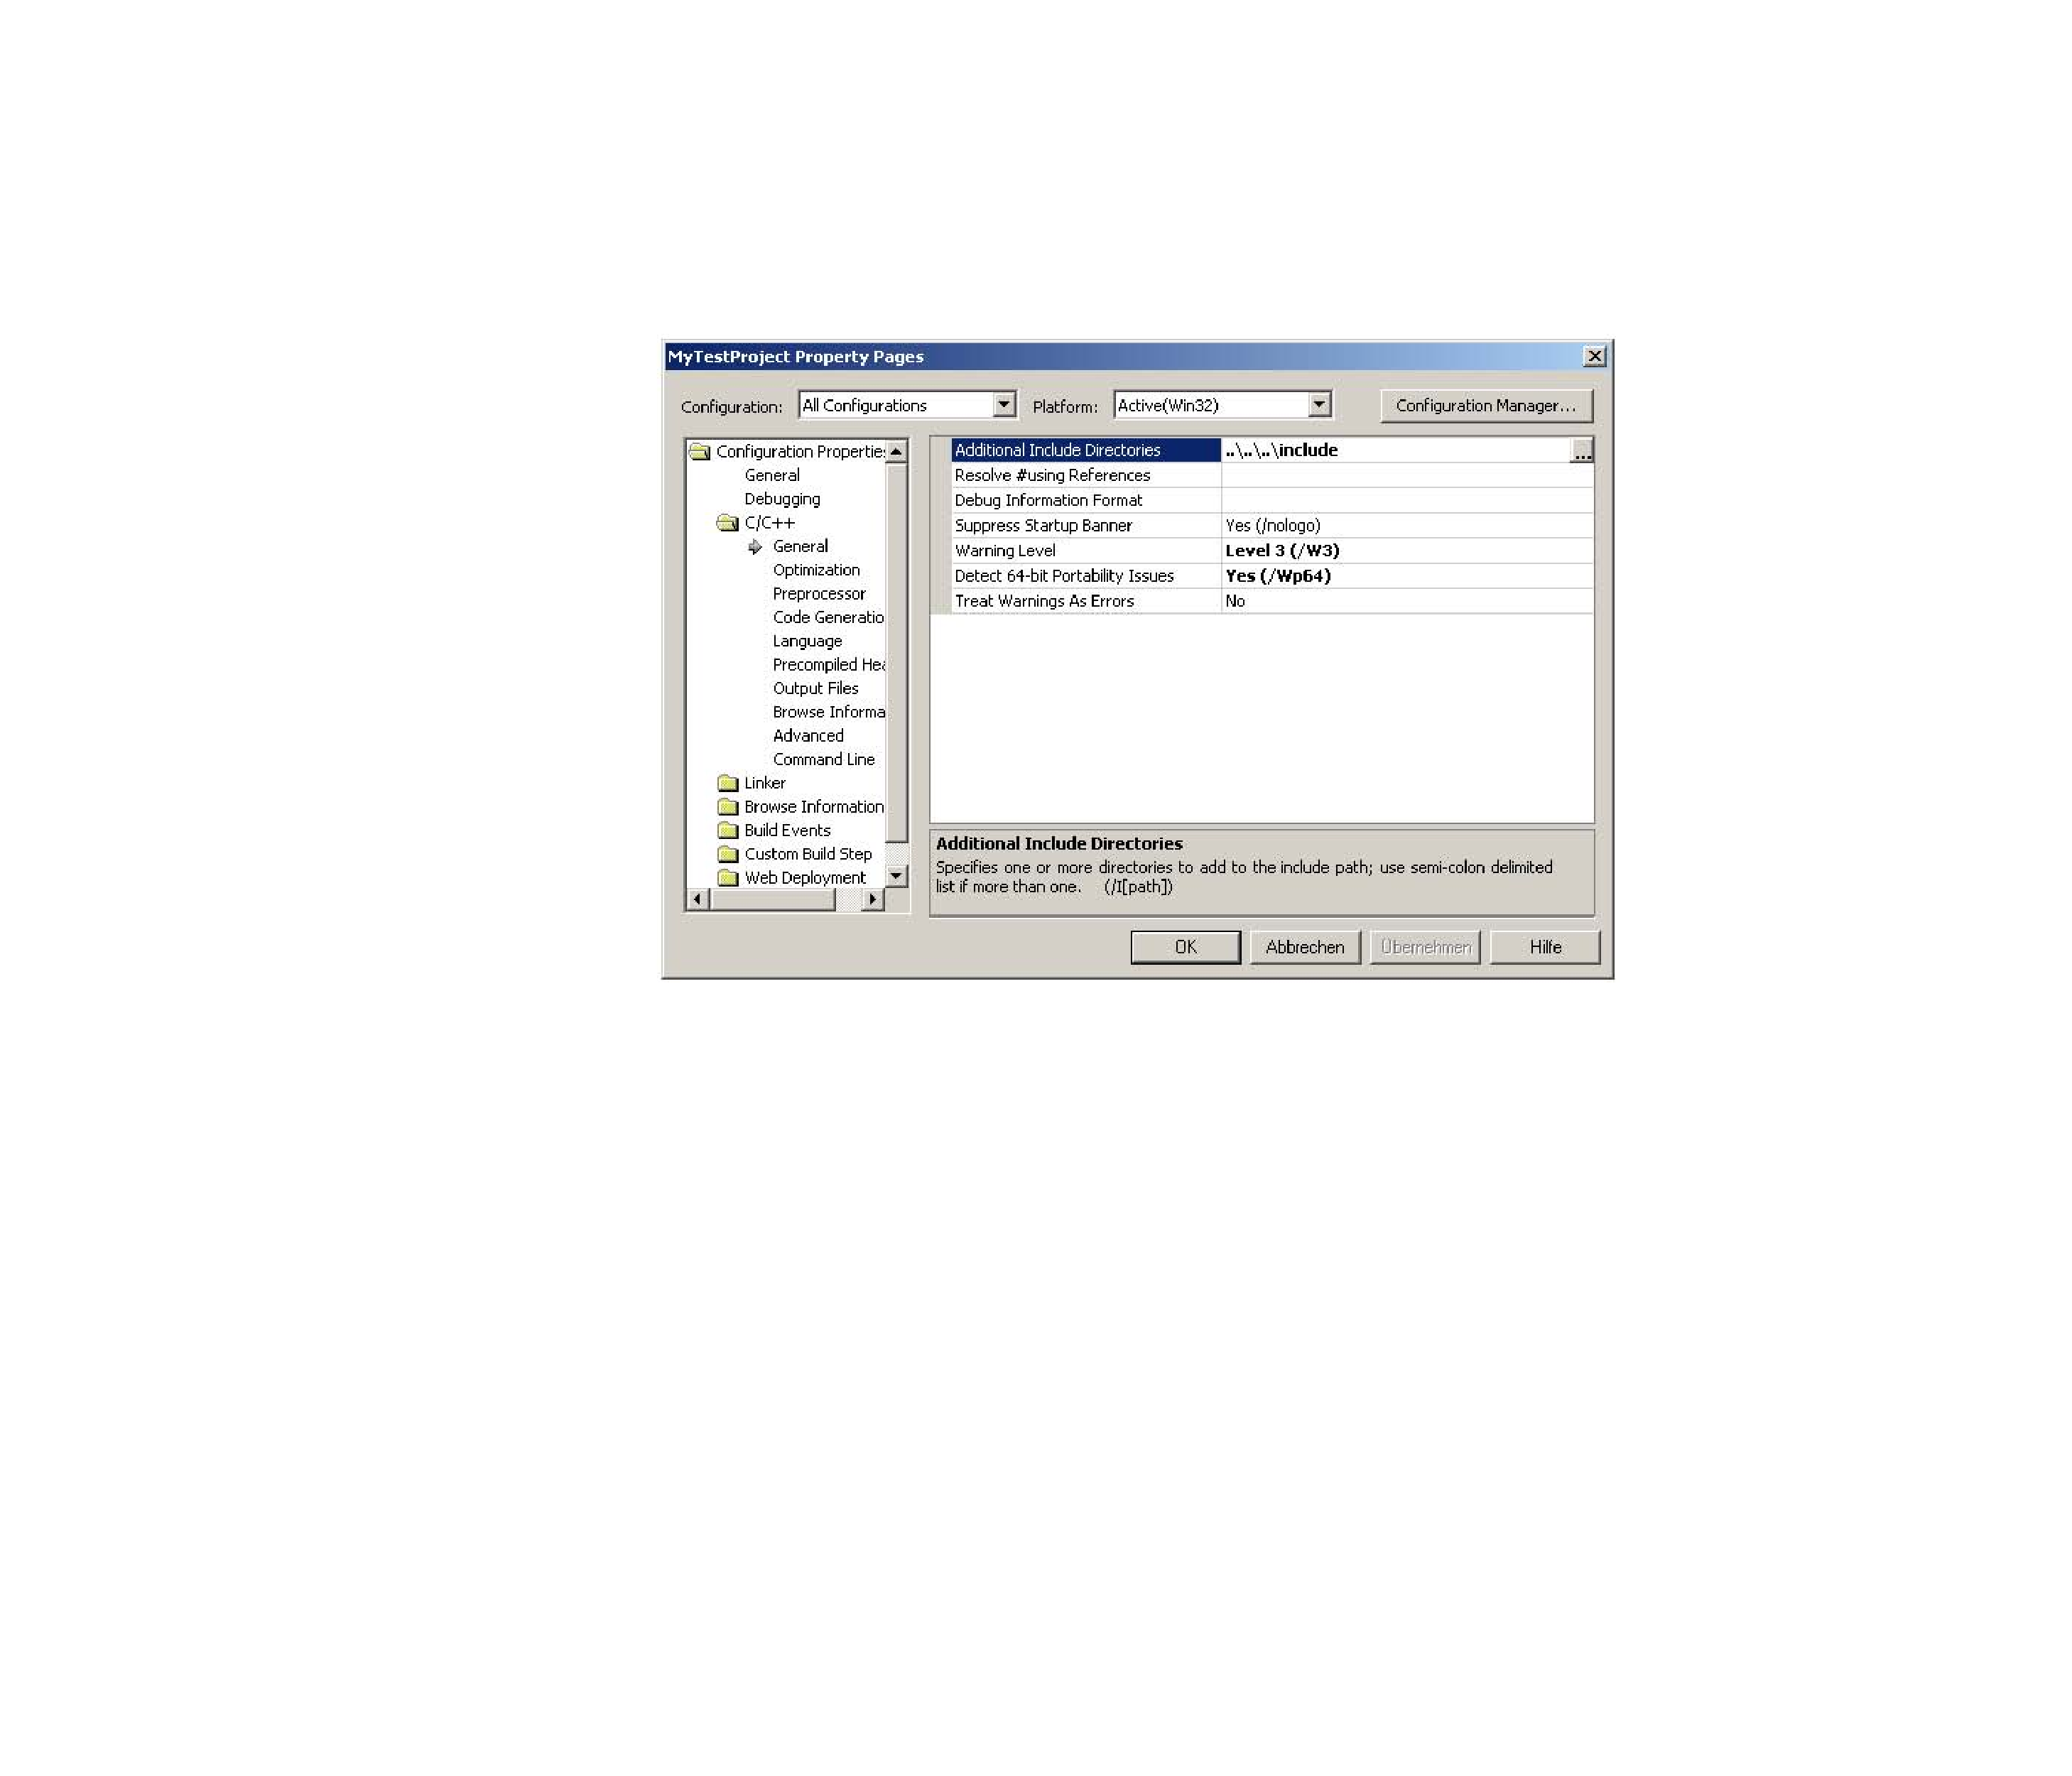
\includegraphics[scale=0.4]{figures/net_setup9.pdf}
\end{center}

TPIE needs to know about the TPIE library file \texttt{tpie.lib} and
its location. This information can be set by opening the ``Linker''
entry and accessing its subentries. The ``General'' subentry provides
the means to set the ``Additional Library Directory'' to
``\path"..\..\..\lib"''.

\begin{center}
  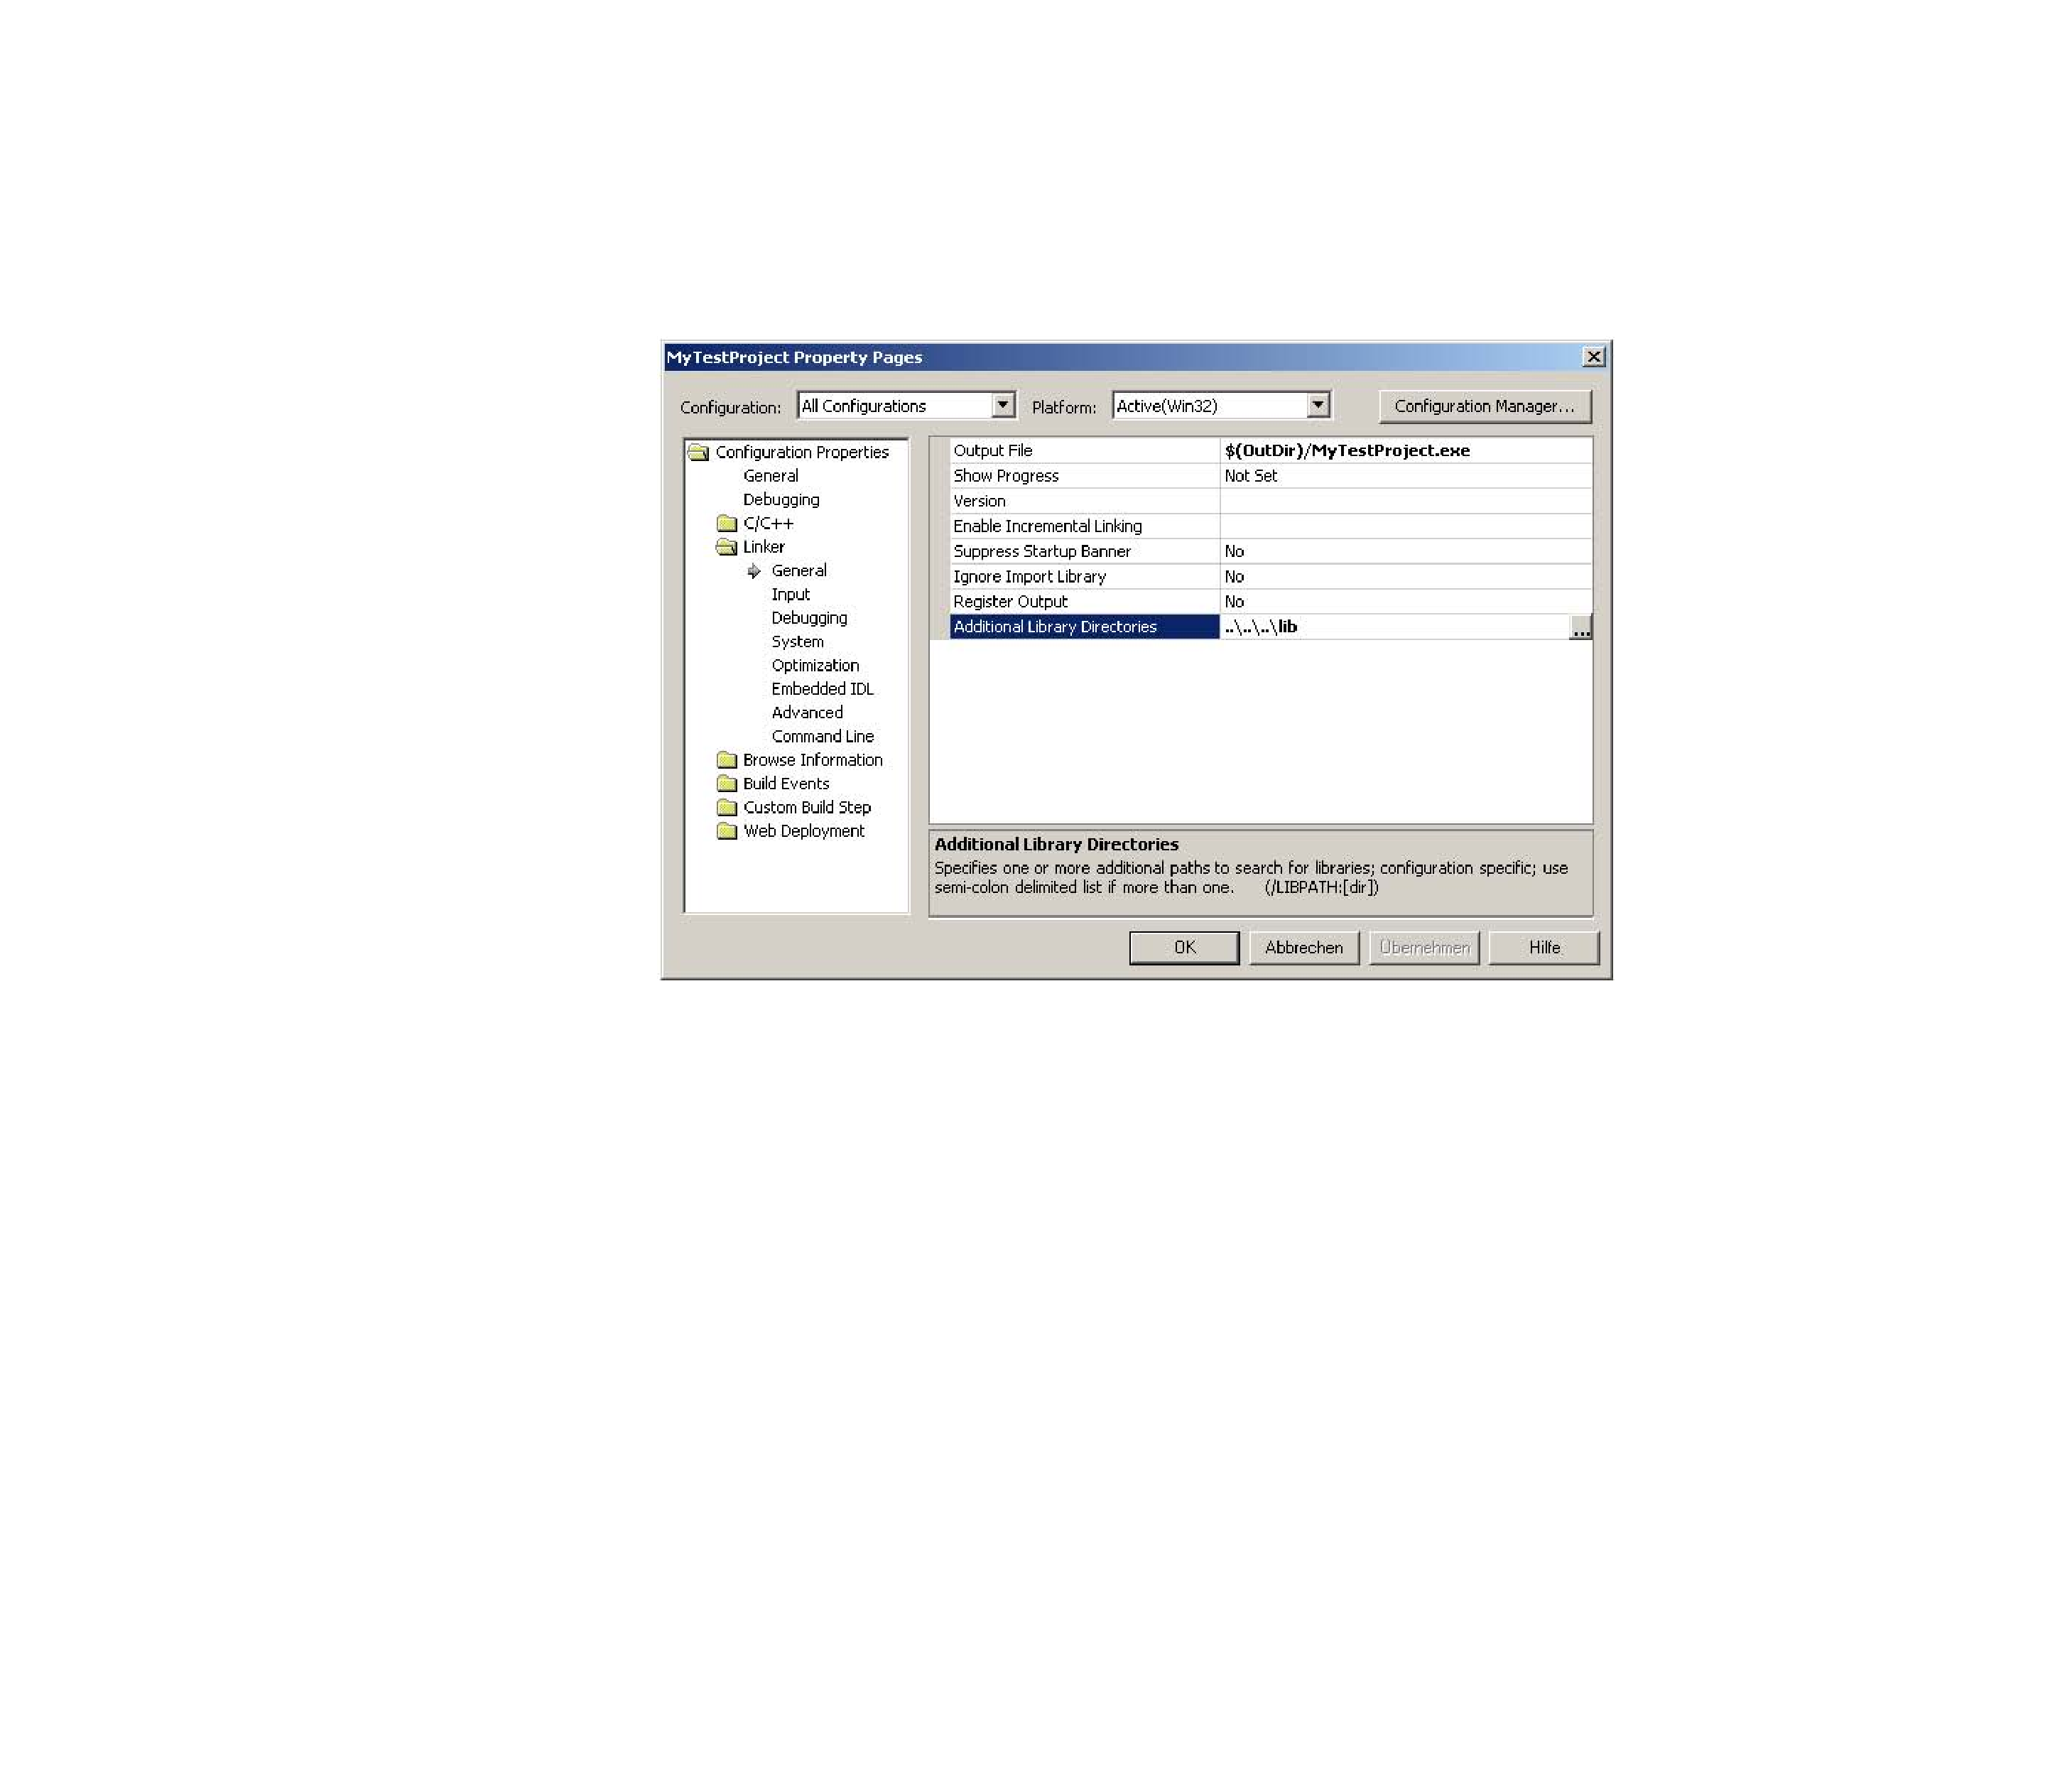
\includegraphics[scale=0.4]{figures/net_setup6.pdf}
\end{center}

The ``Input'' subentry provides means to force linking against the
TPIE library (by setting ``Additional Dependencies'' to
\texttt{tpie.lib}) and for also excluding to link
against�\texttt{libc} (by setting ``Ignore Specific Library'' to
\texttt{libc}). The latter setting is needed to prevent conflicts
between the standard \texttt{new}-operator and TPIE's memory
management. 

\begin{center}
  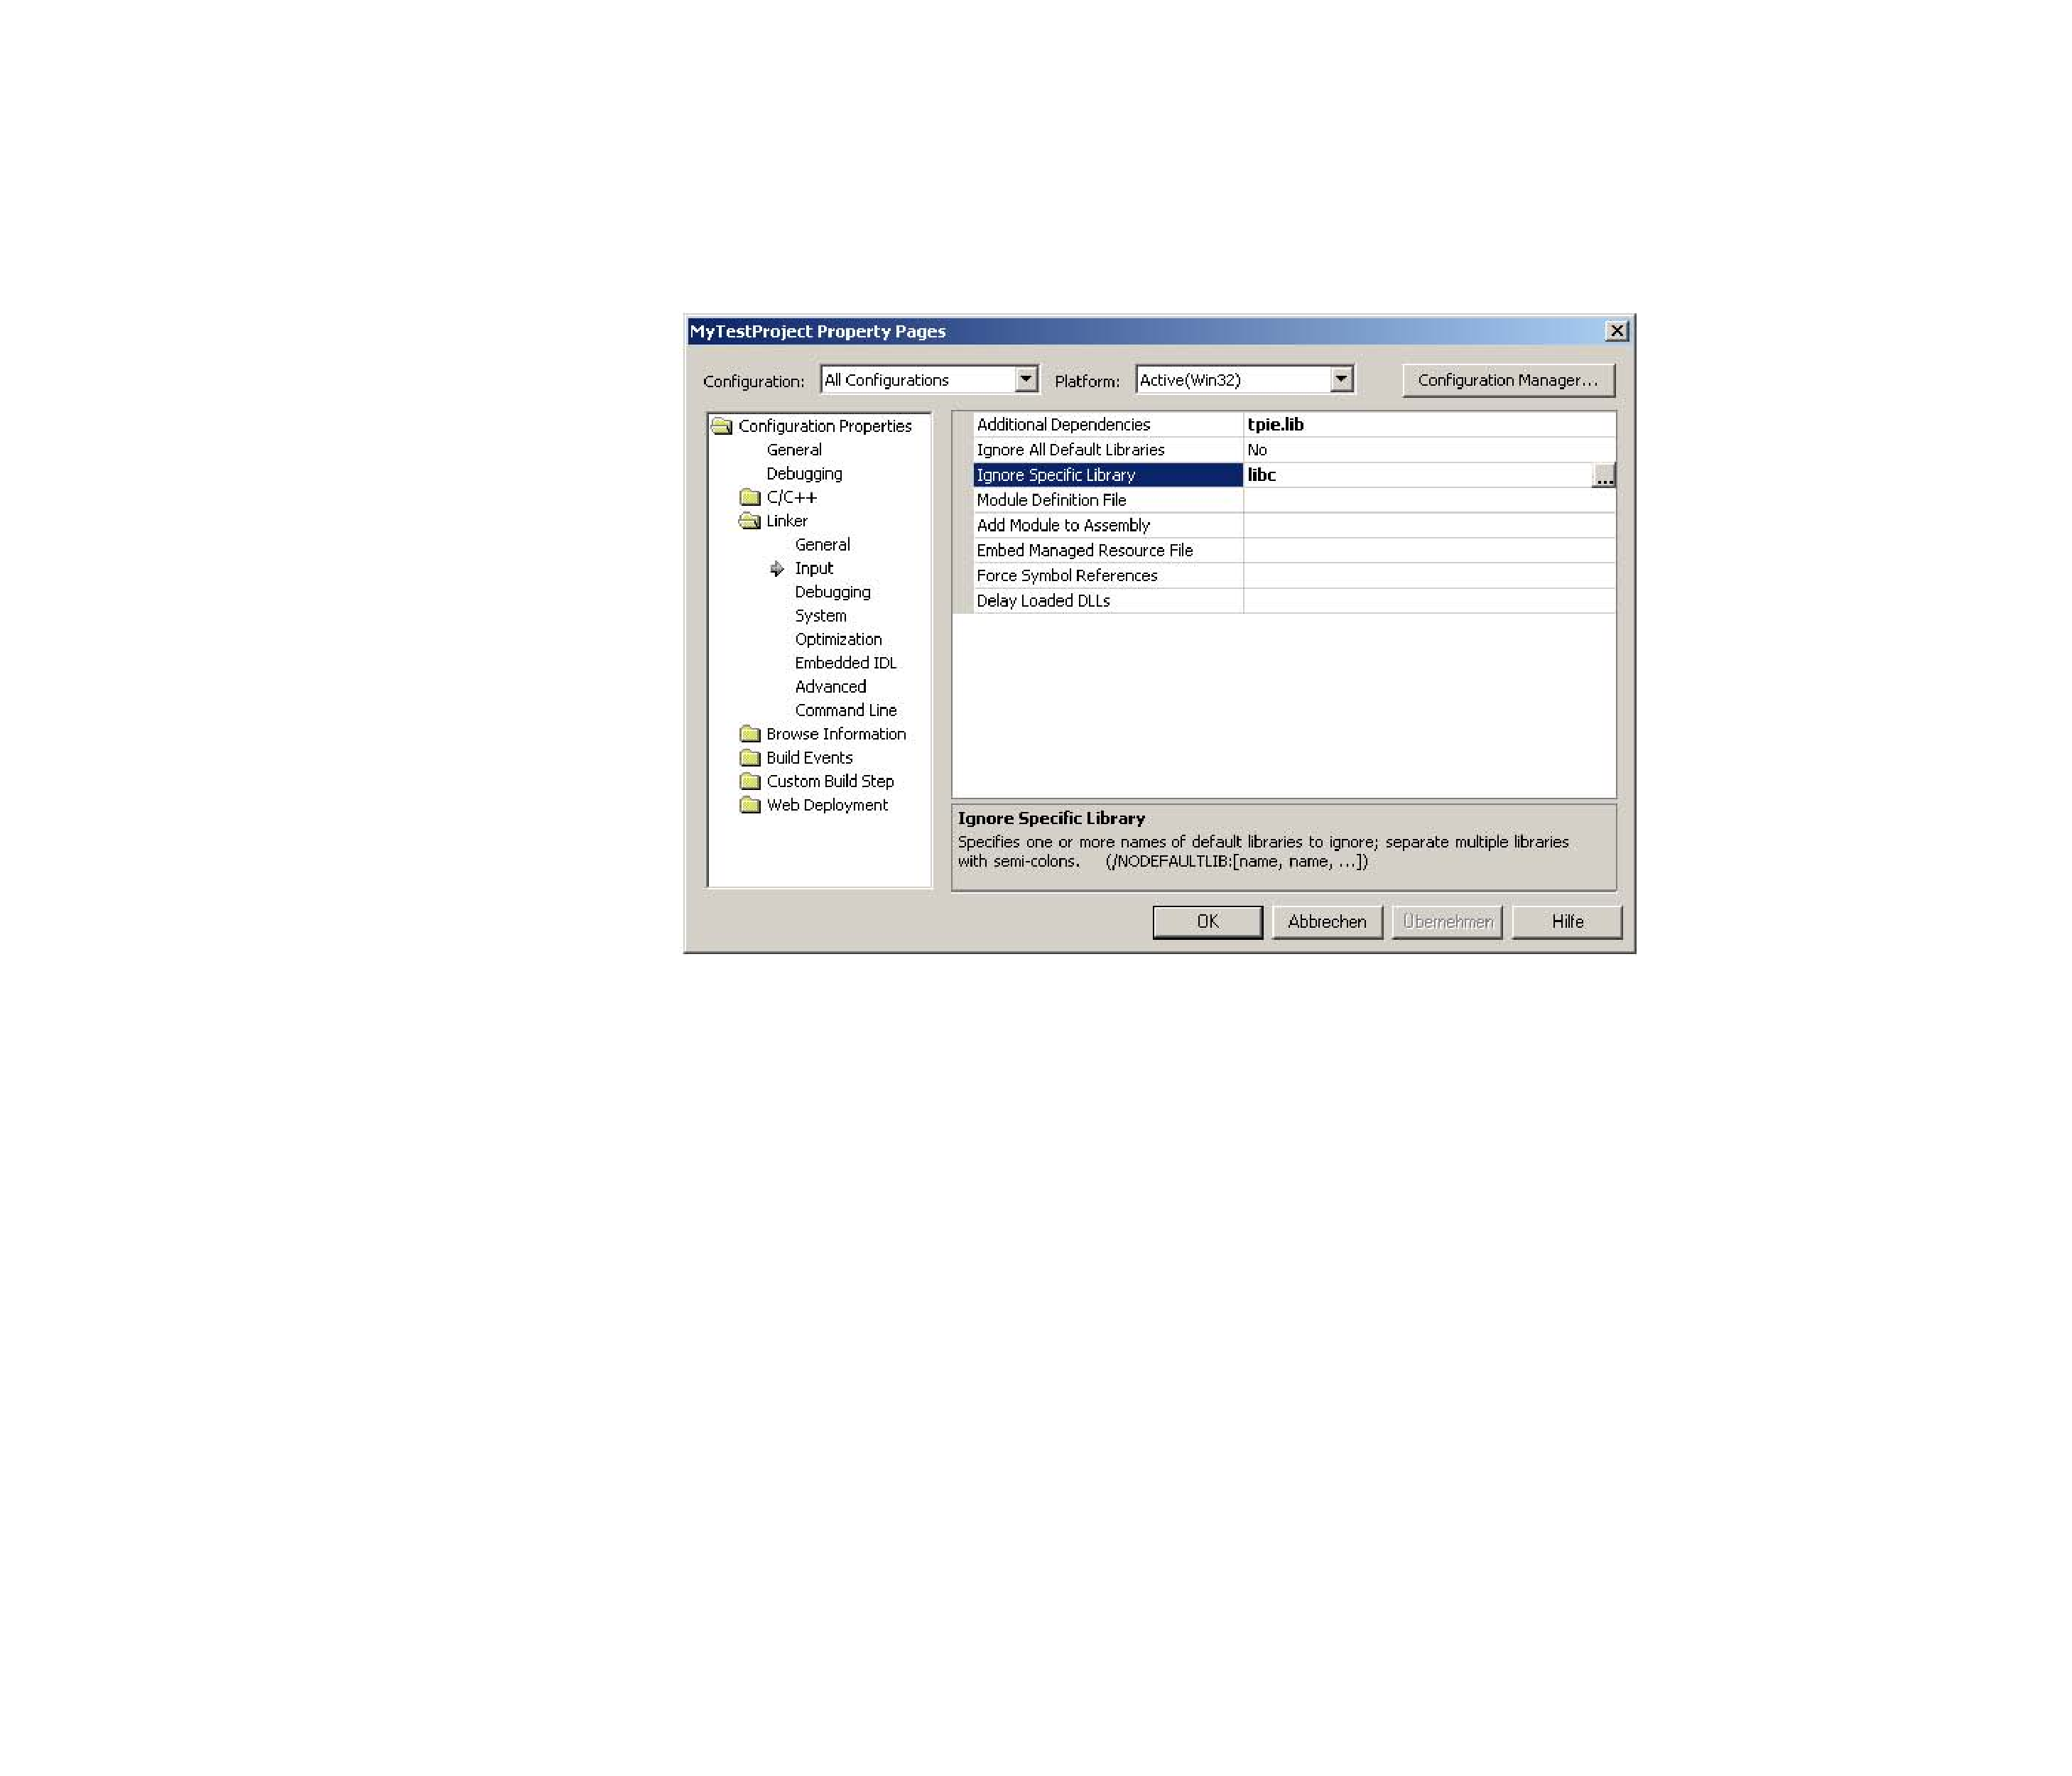
\includegraphics[scale=0.4]{figures/net_setup7.pdf}
\end{center}

Finally, the output directory, i.e., the directory where the compile
will put the executables, has to be set. To maintain executables for
all configurations, this step has to be done seperately for the
``Release'' and the ``Debug'' configuration, and we describe the
process only for the latter. First, select ``Debug'' from the
``Configuration'' pulldown menu, and then select the ``General'' entry
from the left-hand side of the dialog box. In the ``Output
Directory'', enter ``\path"..\..\..\bin\Debug"'', and in the
``Intermediate Directory'', enter ``\path".\Debug"''. Confirm by
clicking ``Ok'' and analogously proceed for the ``Release''
configuration.

\begin{center}
  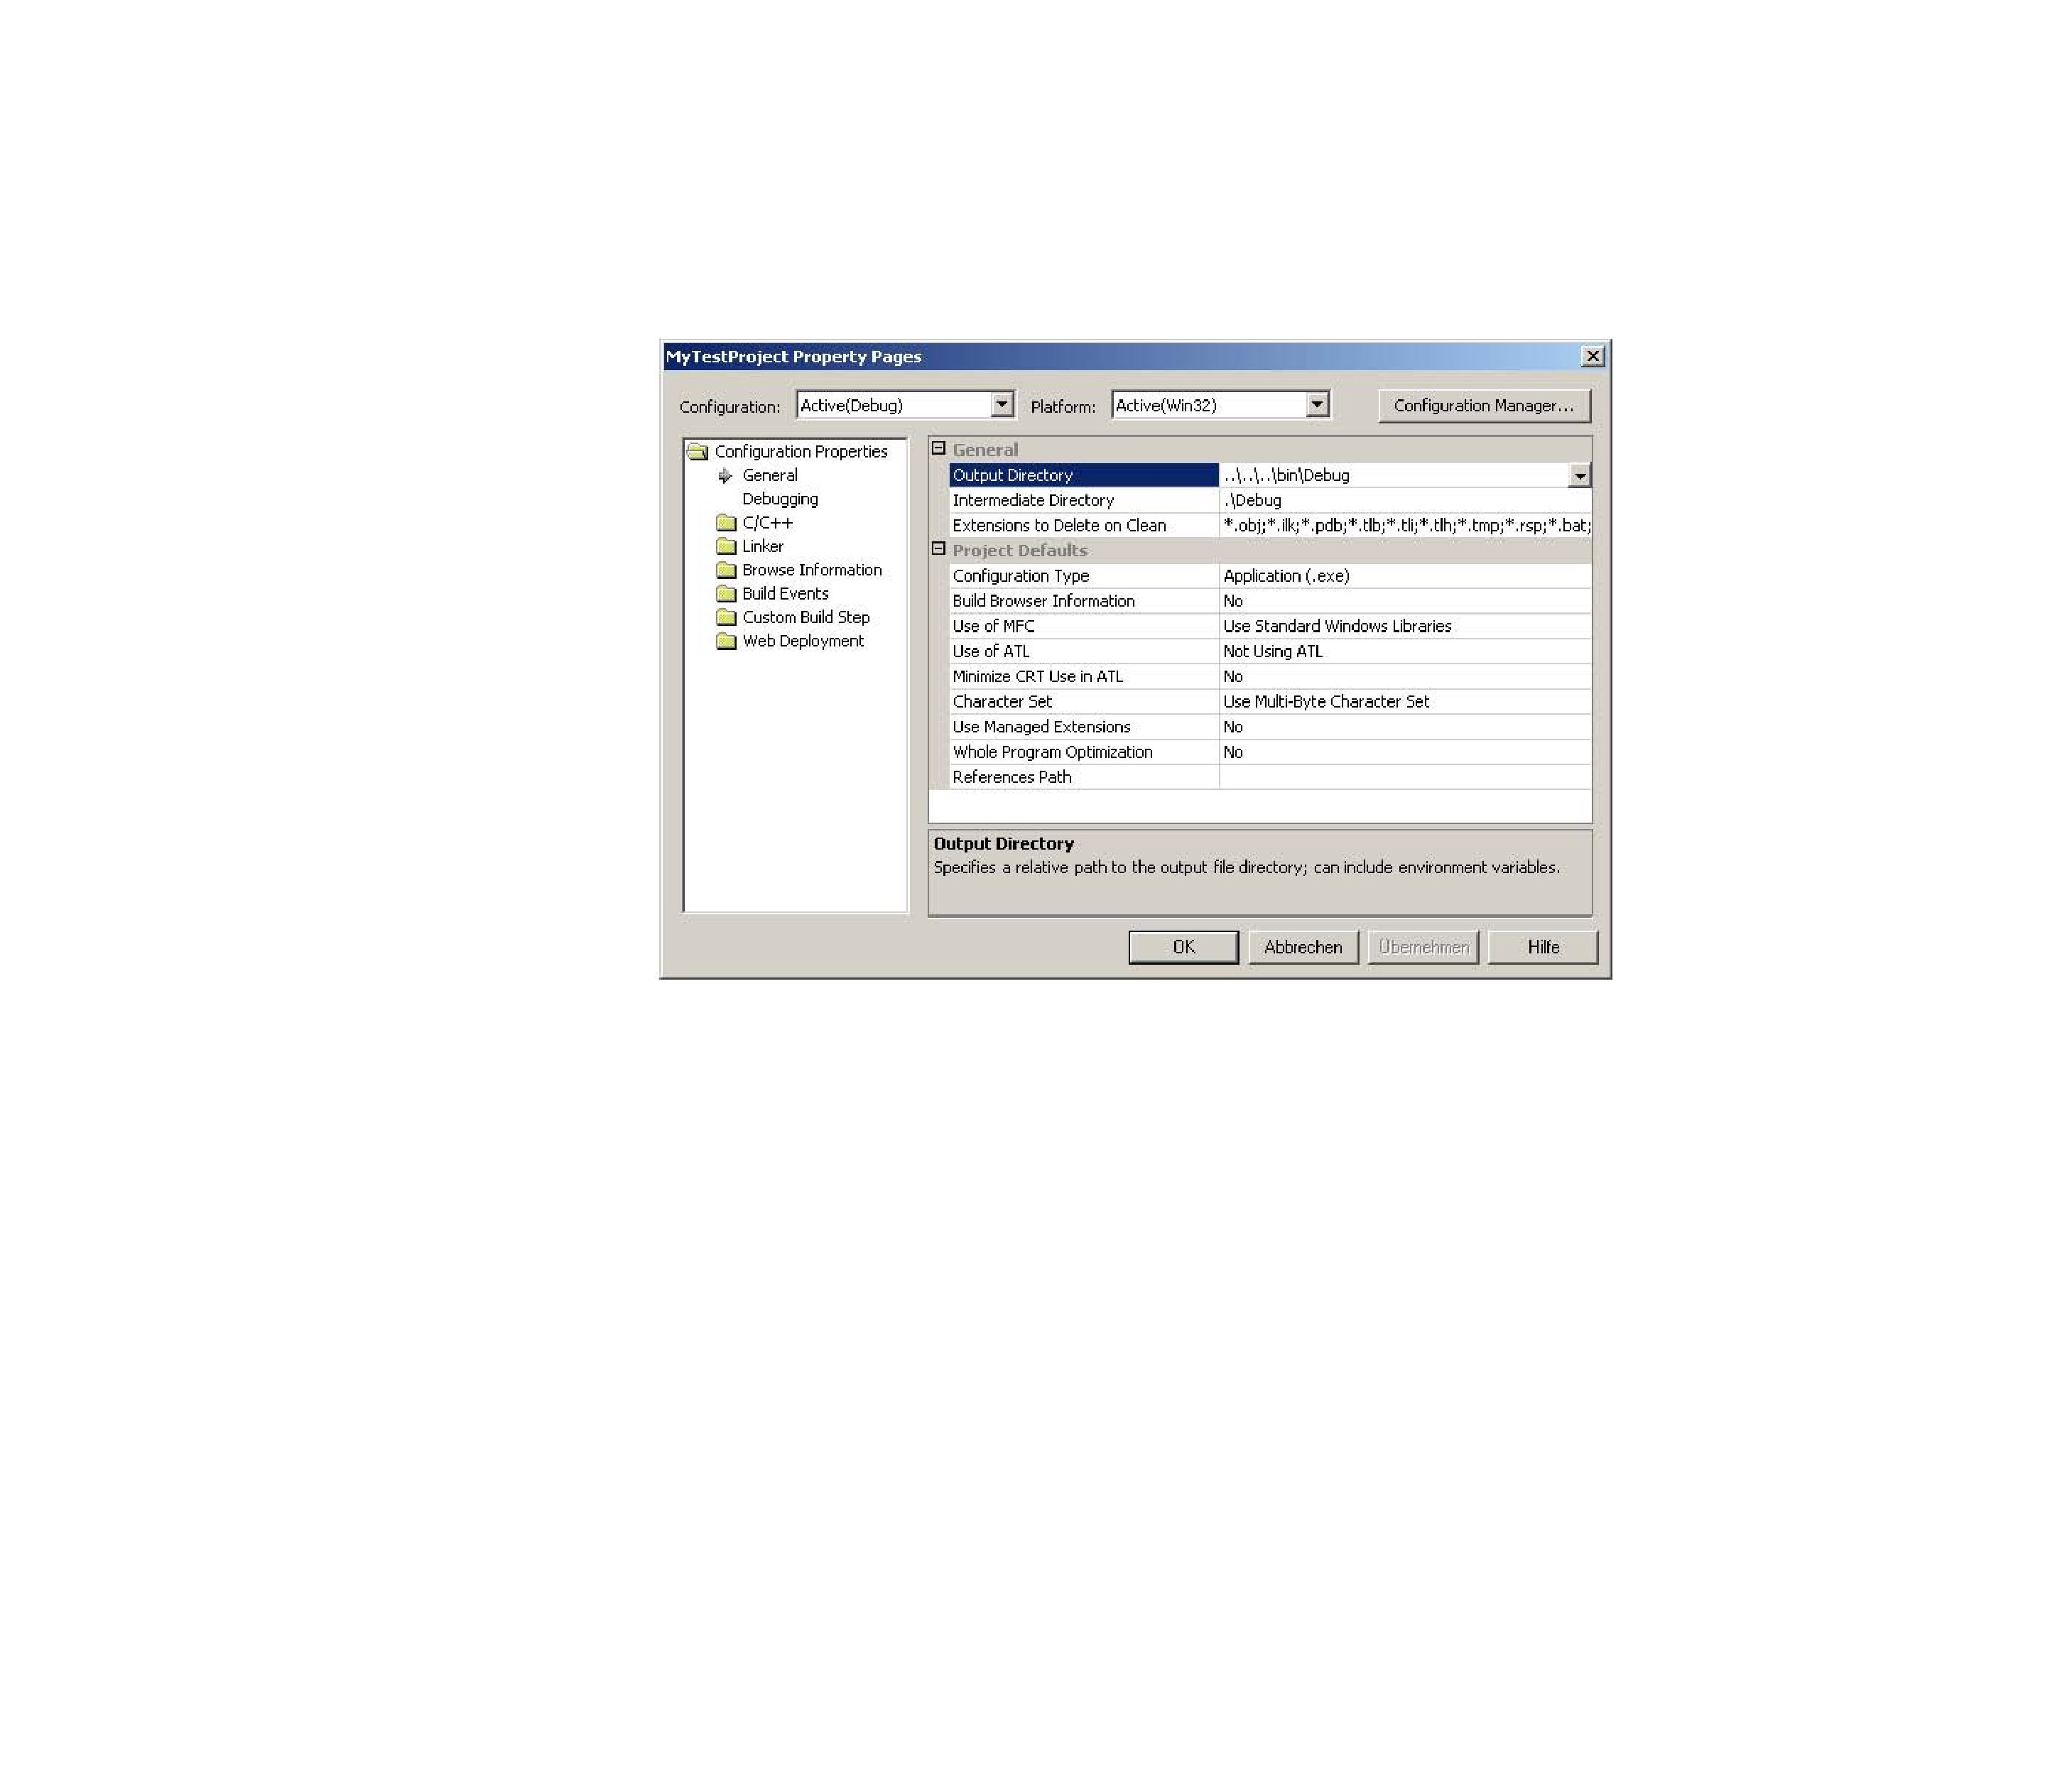
\includegraphics[scale=0.4]{figures/net_setup5.pdf}
\end{center}

You should be ready to proceed with the steps described in the next
chapter of this manual.

\chapter{A Taste of TPIE via a Sample Program}
\plabel{ch:samplepgmr}

\tobewritten(Block oriented part of TPIE)\comment{LA: Add block
  collection example}

This chapter presents a quick look at TPIE via a simple TPIE program.
A more detailed TPIE tutorial appears in Chapter \ref{ch:tutorial}.

One of the primary themes in TPIE is to allow a user to specify an I/O
efficient computation via high-level coordination of data movement
interspersed with appropriate internal memory computing, with the low
level I/O details being transparent, or ``under the hood''.  TPIE
provides various classes of ``management objects'', (e.g. \emphd{scan
  management objects}, \emphd{merge management objects}, etc.) that
allow the user to specify sophisticated data movement operations on
\emphd{streams} of data in a simple and straightforward manner. These
management object classes are built on top of a simple \emphd{stream
  interface} called \lstinline|AMI_STREAM|. The tutorial in the next
chapter explains how to specify and use such management object
classes.

%Using the sample example program below, we take a look at TPIE from a
%viewpoint just above the \lstinline|AMI_STREAM| interface.  
The sample program below uses simple stream
operations\comment{DH: %
   we use only STREAM member functions in the sample
   program, but never describe them in the tutorial. We
   should either describe them or illustrate the power of
   TPIE using operation management objects (scanning,
   merging, sorting, etc.} %
to generate a stream of random integers, scans this stream
of integers and partitions them into several distinct
streams. The manner in which I/O operations are handled by
TPIE ensures that the program is I/O efficient.

%Note that a 4-way distribution can easily be specified using an
%appropriately defined scan management object (see
%Section~\ref{sec:tut-scanning}), in which case the user does not have to use
%stream operations.

The intent of this example is to illustrate the sort of things
involved in TPIE programming; the typical include files, specifying
how much memory the program should use, streaming operations, etc. The
program is given in Section~\ref{sec:tut-samplepgm} and it is
discussed in Section~\ref{sec:tut-samplepgm-discuss}.


\section{Sample Program}\plabel{sec:tut-samplepgm}
\index{sample program|(}
\index{sample program|)}

The following sample program can be found in
\texttt{tpie\_\version/test/sample\_pgm.cpp} after TPIE has been
installed (see Section \ref{sec:tut-installation} of this manual for
installation instructions).

\lstinputlisting[numbers=left,basicstyle=\ttfamily\small,caption={Code taken from \texttt{tpie\_\version/test/sample\_pgm.cpp}}]{src/sample_pgm.cpp}

\section{Discussion of Sample Program}\plabel{sec:tut-samplepgm-discuss}

In\comment{LA: Jan do we need something about portability here?} this
section we discuss the simple \CPP{} sample program shown in the
previous section. The file \path"app_config.h" is the TPIE
configuration file. TPIE's \lstinline|AMI_STREAM| stream I/O
operations are carried out transparently by one of three possible
\emphd{block transfer engines (BTEs)}. Briefly, the file
\path"app_config.h" chooses a specific BTE, and the amount of internal
memory used as buffer space for each \lstinline|AMI_STREAM|. The
\path"app_config.h" configuration file is further discussed in
Section~\ref{sec:tuning} which also contains a discussion of how to
choose a BTE for a given platform. The file \path"ami.h" contains
TPIE's templated classes and functions, while the file
\path"quicksort.h" contains various quicksort polymorphs. Note that
each \lstinline|AMI_STREAM| corresponds to an underlying Unix file.

The program illustrates the use of the basic \lstinline|AMI_STREAM|
member functions \lstinline|seek()|, \lstinline|read_item()|,
\lstinline|write_item()|, and \lstinline|persist()|.  Successful
execution of these member functions is indicated by a return value of
\lstinline|AMI_ERROR_NO_ERROR|.  The program distributes a randomly
generated source stream of integers into eight bucket streams, and
then displays the time taken by this operation and the size of each of
the eight output buckets. The randomly generated stream is deleted
upon completion of the program
(\lstinline|source.persist(PERSIST_DELETE)|), while the bucket streams
are saved (made persistent with
\lstinline|buckets[i].persist(PERSIST_PERSISTENT)|) in the default
scratch directory \path"/var/tmp/". The default location for the
scratch files can be changed by setting the environment variable
\lstinline|AMI_SINGLE_DEVICE| appropriately (see
Section~\ref{sec:environment}).

TPIE can run with a user-specified amount of internal memory (although
typically, about 4~MB is required as a minimum for most simple
applications) or it can run with virtual memory like an ordinary
non-TPIE application. The former mode is invoked by calling
\lstinline|MM_manager.ignore_memory_limit()|, and the latter by
calling \lstinline|MM_manager.enforce_memory_limit()|.

In the sample program, we call
\lstinline|MM_manager.enforce_memory_limit()|, which means that the
program will abort if the allocated internal memory exceeds the
specified amount. The successive function call
\lstinline|MM_manager.set_memory_limit(test_mm_size)| tells TPIE's
internal memory manager \lstinline|MM_manager| to prevent the
program's internal memory usage from exceeding
\lstinline|test_mm_size| bytes (\lstinline|test_mm_size| is the second
input argument to our program). When
\lstinline|MM_manager.enforce_memory_limit()| is used, it is the
responsibility of the user to inform \lstinline|MM_manager| via
\lstinline|set_memory_limit()| of the desired memory limit.  For
example, one might set this value to the amount of physical main
memory minus the main memory used by the operating system and other
programs running on the machine.

%In the case of the present program, it is desirable to
%ensure that the program is allowed enough memory to comfortably accommodate
%the buffer space required by each one of the nine \lstinline|AMI_STREAM|s
%involved in the computation. The amount of buffer space required per
%\lstinline|AMI_STREAM| depends on the BTE implementation chosen in the
%\path"app_config.h" file. Section~\ref{sec:env-variables} provides details
%of how to determine the buffer-space required for each BTE implementation.

The sample program can be compiled as follows: (recall that Section
\ref{sec:tut-gnu-software} discussed the version of GNU \CPP{}
required):

\begin{lstlisting}
cd test
make sample_pgm
\end{lstlisting}

By way of example, the program can be run with 1000000 random integers
and 5000000 bytes of main memory as follows:
\begin{lstlisting}
cd ../bin
sample_pgm 1000000 5000000
\end{lstlisting}


\chapter{Tutorial}
\plabel{ch:tutorial}

\tobewritten(Block oriented part of TPIE)

\section{Introduction}\plabel{sec:tut-introduction}

This tutorial is designed to introduce new users to the TPIE system.
It introduces the fundamental paradigms of computation that TPIE
supports, giving source code examples of each.  The majority of the
code presented in the tutorial is available in the test
applications\index{test applications} directory of the distribution,
\texttt{tpie\_\version/test/}.

For the sake of brevity, much of the code presented in this tutorial
is incomplete, in the sense that necessary header files \index{header
  files} and macros\index{macros} are omitted. Details concerning how
to write your own complete TPIE code is presented at the end of the
tutorial in Section~\ref{sec:tut-compiling} (see also
Sections~\ref{ch:samplepgmr} and \ref{sec:choosingbte})\comment{LA:
  Maybe we should talk briefly about AMI, BTE, MM somewhere around
  here - we talk about main memory issues in merging and compiling
  sections.}

TPIE is written in the \CPP{} language, and this manual assumes that
the reader is familiar with \CPP{}.  If you would like to use TPIE but
are not familiar with the \CPP{}\index{C++} language, a number of good
books are available.\comment{LA: Update?} If you are familiar with
C\index{C}, \cite{pohl:c++} is a good place to start. A more basic,
but very comprehensive book is~\cite{deitel:c++}, and
\cite{meyers:effective} is an excellent source of information on
intermediate and advanced \CPP{}.  Finally, \cite{ellis:arm} is the
definitive book on \CPP{}, though not necessarily the best place for
new programmers to start.

Familiarity with the theoretical results on I/O-efficient algorithms
is not necessary in order to use TPIE. However, this tutorial (and the
rest of this manual) may be easier to follow with some general
background information such as how a theoretically optimal external
(merge) sort algorithm works. Good references
are~\cite{vitter:iosurvey, arge:handbook}. Some of the basic concepts
required for understanding the discussion of I/O issues and external
memory algorithms in this manual are outlined in
Section~\ref{sec:tut-concepts}.

\section{Basic Concepts}\plabel{sec:tut-concepts}
\index{concepts}\index{basic concepts}
   
Roughly speaking there is a factor of a million difference in the
access time of internal and external memory.  In order to cope with
the high cost of accessing externally-stored data, efficient EM
algorithms exploit locality in their design.  They access a large
\emphd{block} of $B$ contiguous data elements at a time and perform
the necessary algorithmic steps on the elements in the block while it
is in the high-speed memory. The speedup can be considerable.  A
second effective strategy for EM algorithms is the use of multiple
parallel disks; whenever an input/output operation is performed, $D$
blocks are transferred in parallel between memory and each of the $D$
disks (one block per disk).

The performance of an EM algorithm on a given set of data is affected
directly by how much internal memory is available for its use. We use
$M$ to denote the number of application data elements that fit into
the internal memory available to the algorithm, and $m=M/B$ denotes
the number of blocks that fit into the available internal memory. Such
a block is more precisely called a \emphd{logical block} because it
may be a different size (usually larger) than either the physical
block size or the system block size. We will reserve the term
\emphd{physical block} size to mean the block size used by a disk
controller to communicate with a physical disk, and the \emphd{system
  block} size will be the size of block used within the operating
system for I/O operations on disk devices. In EM algorithms we will
assume that the logical block size is a multiple of the system block
size. In TPIE, for instance, this factor is currently set to 32 if not
changed by the user.

TPIE is implemented as a set of templated classes and functions in
\CPP{}, and employs an object-oriented abstraction to EM computation.
TPIE provides \CPP{} templates of various optimal EM computation
\emphd{patterns} or \emphd{paradigms}.  Examples of such paradigms are
the EM algorithms for merge sorting, distribution sweeping, time
forward processing, etc. (see \cite{vitter:dimacssurvey}). In a TPIE
program, the application programmer provides application-specific
details of the specific computation paradigm used, such as \CPP{}
object definitions of the application data records, and code for
application-specific sub-computations at critical points in the
computation pattern, but TPIE provides the application-independent
parts of the pattern.

The definition of an application data element (or record) is provided
by the user as a class definition.  Such a class definition is
typically used as a template parameter in a TPIE code fragment (e.g. a
templated function). Other template parameters may be instantiated by
choices the user makes between algorithm options (e.g. between sorting
variants) or between operating system interfaces (e.g. the choice of
BTE)\comment{LA: Does reader know what BTE is?} for instance. These
user selections allow a pattern replesented by a templated \CPP{} code
fragment to be instantiated as an actual piece of executable code,
tailored to the data types required by the user's application.

Application-dependent sub-computations (e.g. a comparison object used
to determine the order of two application data elements during a sort)
are typically structured as methods of an \emphd{operation management
  object}. TPIE dictates the names and required functionality of each
method of an operation management object, but the details of the
computation performed by a specific method are application-specific
and thus are the responsibility of the application programmer.


\section{Streams}\plabel{sec:tut-streams}
\index{stream}\index{structure!of streams} 

In\comment{LA: something in this section about persistence, read/write
  primitives?}  TPIE, a \emphd{stream} is an ordered collection of
objects of a particular type, stored in external memory, and accessed
in sequential order. Streams can be thought of as fundamental TPIE
objects which map volatile, typed application data elements in
internal memory to persistent, untyped data elements in external
memory, and vice-versa.  Streams are read and written like files in
Unix and support a number of primitive file-like operations such as
\lstinline|read()|, \lstinline|write()|, \lstinline|truncate()|, etc.
%See Section \ref{implementationofstreams} for more
%information.
TPIE also supports the concept of a \emphd{substream}, which
permits a contiguous subset of the elements in a stream to
accessed sequentially. Multiple substreams can be created on
streams and even on other substreams. 
%Substreams are deprecated in TPIE due to performance issues
%(see Section \ref{substreams} for more information).

Various paradigms of external memory computation are supported on
streams (and substreams) in TPIE, including scanning (see Section
\ref{sec:tut-scanning}), merging (see Section \ref{sec:tut-merging}),
and sorting (see Section \ref{sec:tut-sorting}). TPIE reduces the
programming effort required to perform an external sort, merge, etc.,
by providing the high level flow of control within each paradigm, and
therefore structuring this part of the computation so that it will be
I/O efficient. The programmer is left with the task of providing what
amount to ``event handlers'', specifying the application-specific
details of the computation. For instance in sorting, the programmer
defines a stream of input data, a comparison object (the event handler
for the task of comparing two application data elements), and an
output stream for the results. In TPIE terminology, the collection of
necessary event handlers for a particular EM computational paradigm is
contained in an \emphd{operation management object}. Operation
management objects differ according to which paradigm is used.  See
Section \ref{sec:tut-scanning} for a discussion of scan management
objects, Section \ref{sec:tut-merging} for a discussion of merge
management objects, and Section \ref{sec:tut-sorting} for a discussion
of sort management objects.\comment{LA: We don't have a sort
  management object anymore do we?! AD: We do, but it is never used
  directly.}

Creating a stream of objects in TPIE is very much like creating any
other object in \CPP{}. The only difference is that the data placed in
the stream is stored in external memory (on disk).
%In some respects this aspect of TPIE can
%be viewed as an implementation of \emphd{persistent objects}
%(see Section~\ref{BCCstuff} for more discussion of persistent objects).
For example, to create an (empty) stream \lstinline|stream0| capable
of storing integers, we could use the following:
\begin{lstlisting}
AMI_STREAM<int> stream0;
\end{lstlisting}
Alternatively, the following creates a pointer
\lstinline|p| to an empty stream of \lstinline|applrec| objects:
\begin{lstlisting}
AMI_STREAM<applrec> *p = new AMI_STREAM<applrec>;
\end{lstlisting}

The \lstinline|AMI| prefix in \lstinline|AMI_STREAM| stands for
\emphd{Access Method Interface}\index{Access Method Interface
  (AMI)}\index{AMI}. This layer of TPIE contains the services and
functionality which a normal user of TPIE will require.
(\lstinline|AMI_STREAM| is actually a compile-time macro that
evaluates to the name of a particular implementation of streams, but
for now it is safe to assume that it is simply a \CPP{} class).

The \lstinline|AMI_STREAM| constructor does not actually put anything
into the stream; it simply creates the necessary data structures to
keep track of the contents of the stream when data is actually put
into it.  One basic way of putting data into a stream is via
\lstinline|AMI_scan()|, which is described in Section
\ref{sec:tut-scanning}.


\section{Operation Management Objects} 
\plabel{sec:tut-omos}\index{operation management object}

TPIE\comment{LA: This first paragraph seems to be repeat and the rest
  I don't know why is there. Remove whole section?} provides a
structure for performing a number of basic operations, such as
scanning a stream of items, merging streams of items, sorting a stream
of items, etc. Much of the application-independent work in these
operations is handled by TPIE.  The TPIE user, however, must provide
the code for the application-dependent aspects of these operations via
a TPIE {\em operation management object}. An operation management
object in TPIE is an object which contains member functions to control
the critical, application-varying aspects of operations such as
scanning, merging, and sorting. TPIE expects certain named methods of
the object to be present, depending on the operation being performed.

The operation management object for scanning (called a ``scan
management object''\index{operation management object!scan}), for
instance, must provide methods \lstinline|initialize| (for
initializing any user-required data structures of the scan), and
\lstinline|operate| (for performing whatever steps are needed as each
data item is encountered in the scan). See Section
\ref{sec:tut-scanning} below for more information.

In the example of merging, the rules for ``combining'' elements of the
merge operation are necessarily application dependent. TPIE expects a
``merge management object''\index{operation management object!merge}
to contain members \lstinline|initialize| and \lstinline|operate|, as
well as several others. Detailed requirements for merge management
objects are described in Section \ref{sec:tut-merging}.

\section{Scanning}
\plabel{sec:tut-scanning}

\index{scanning|(} \index{AMI_scan()@{\tt AMI\_scan()}} The simplest
paradigm available in TPIE is scanning.  Scanning can be used to
produce streams, examine the contents of streams, or transform
streams.

\subsection{Basic Scanning}

One basic thing a scan can do is write a series of objects to a
stream.  In the following example, we create a stream of integers
consisting of the first 10000 natural numbers.

\lstinputlisting[basicstyle=\ttfamily\small,firstline=20,lastline=47]{src/scan_count.cpp}

The object \lstinline|sc| is called a scan management
object\index{operation management object!scan}.  It has two member
functions, \lstinline|initialize()| and \lstinline|operate()|, which
TPIE calls when asked to perform a scan.  The first member function,
\lstinline|initialize()| is called at the beginning of the scan.  TPIE
expects that a call to this member function will cause the object to
initialize any internal state it may maintain in preparation for
performing a scan.  The second member function, \lstinline|operate()|,
is called repeatedly during the scan to create objects to go into the
output stream.  \lstinline|operate()| sets the flag \lstinline|*sf| to
indicate whether it generated output or not.  TPIE will call
\lstinline|operate()| as long as \lstinline|operate()| returns
\lstinline|AMI_SCAN_CONTINUE|. The normal way for
\lstinline|operate()| to signal that it is finished is to return the
value \lstinline|AMI_SCAN_DONE|.

\lstinline|AMI_scan| behaves as the following pseudo-code:

\lstinputlisting[basicstyle=\ttfamily\small,firstline=49,lastline=67]{src/scan_count.cpp}

Thus, after the function \lstinline|f()| in the original example code
returns, the stream \lstinline|amis0| will contain the integers from 1
to 10000 in increasing order.

One of the simplest things we can do with a stream of objects is scan
it in order to transform it in some way.  As an example, suppose we
wanted to square every integer in the stream \lstinline|amis0|.  We
could do so using the following code:

\lstinputlisting[basicstyle=\ttfamily\small,firstline=20,lastline=45]{src/scan_square.cpp}

Notice that the call to \lstinline|AMI_scan()| in \lstinline|g()|
differs from the one we used in \lstinline|f()| in that it takes two
stream pointers and a scan management object.  By convention, the
stream \lstinline|amis0| is an input stream, because it appears before
the scan management object \lstinline|ss| in the argument list.  By
similar convention, \lstinline|amis1| is an output stream.  Because
the call to \lstinline|AMI_scan| has one input stream and one output
stream, TPIE expects the \lstinline|operate()| member function of
\lstinline|ss| to have one input argument (which is called
\lstinline|in| in the example above) and one output argument (called
\lstinline|out| in the example above).  Note that the
\lstinline|operate()| member function of the class
\lstinline|square_scan| also takes two pointers to flags, one for
input (\lstinline|sfin|) and one for output (\lstinline|sfout|).
\lstinline|*sfin| is set by TPIE to indicate that there is more input
to be processed.  \lstinline|*sfout| is set by the scan management
object to indicate when output is generated.  A scan management object
must contain an \lstinline|operate()| member function that takes the
appropriate types and number of arguments for the invocation of
\lstinline|AMI_scan()| that uses it, or else a compile-time error will
be generated.

\lstinline|AMI_scan| with one input stream and one output stream
behaves as the following pseudo-code:

\lstinputlisting[basicstyle=\ttfamily\small,firstline=47,lastline=74]{src/scan_square.cpp}

\lstinline|AMI_scan()| can operate on up to four input streams and
four output streams.  Here is an example that takes two input streams
of values, \lstinline|x| and \lstinline|y|, and produces four output
streams, one consisting of the running sum of the \lstinline|x|
values, one consisting of the running sum of the \lstinline|y| values,
one consisting of the running sum of the squares of the \lstinline|x|
values, and one consisting of the running sum of the squares of the
\lstinline|y| values.

\lstinputlisting[numberstyle=\tiny,stepnumber=5,basicstyle=\ttfamily\small,firstline=20]{src/scan_sum.cpp}


\subsection{ASCII Input/Output} \plabel{sec:tut-ascii-io}

\index{ASCII I/O|see{scanning, ASCII I/O}} \index{scanning!ASCII
  I/O|(} TPIE provides a number of predefined scan management objects.
Among the most useful are instances of the template classes
\lstinline|cxx_ostream_scan<T>| and \lstinline|cxx_ostream_scan<T>|,
which are used for reading ASCII data into streams and writing the
contents of streams in ASCII respectively.  This is done in
conjunction with the \lstinline|iostream| facilities provided in the
standard \CPP{} library.  Any class \lstinline|T| for which the
operators \lstinline|ostream &operator<<(ostream &s, T &t)| and
\lstinline|istream &operator>>(T &t)| are defined can be used with
this mechanism.

As an example, suppose we have an ASCII file called
\path"input_nums.txt" containing one integer per line, such as

\begin{lstlisting}
17
289
4195835
3145727
.
.
.
\end{lstlisting}

The following code copies this file into a TPIE stream of integers,
squares each one, and writes the results to the file
\path"output_nums.txt".

\lstinputlisting[basicstyle=\ttfamily\small,firstline=76,lastline=94]{src/scan_square.cpp}

In order to read from an ASCII input file using the scan management
object \lstinline|in_scan|, \lstinline|AMI_scan()| repeatedly calls
\lstinline|in_scan->operate()|, just as it would for any scan
management object.  Each time \lstinline|in_scan->operate()| is
called, it uses the \lstinline|>>| operator to read a single integer
from the input file.  When the input file is exhausted,
\lstinline|in_scan->operate()| returns \lstinline|AMI_SCAN_DONE|, and
\lstinline|AMI_scan()| returns to its caller.  The behavior of
\lstinline|out_scan| is similar to that of \lstinline|in_scan|, except
that it writes to a file instead of reading from one.
\index{scanning!ASCII I/O|)}

\subsection{Multi-Type Scanning}

\index{scanning!multi-type|(}

In all of the examples presented up to this point, scanning has been
done on streams of objects that are all of the same type.
\lstinline|AMI_scan()| is not limited to such scans, however.  In the
following example, we have a scan management class that takes two
streams of \lstinline|double|s and returns a stream of complex
numbers.

\lstinputlisting[basicstyle=\ttfamily\small,firstline=20]{src/complex.cpp}
\index{scanning!multi-type|)}

\subsection{Out of Step Scanning}
\plabel{sec:tut-out-of-step}

\index{scanning!out of step|(} In all the examples up to this point,
the \lstinline|operate()| member function of a scan management object
has been called exactly once for each object in the input stream(s).
In this section, we discuss the concept of out of step scanning, which
involves using a scan management object to reject certain inputs and
ask that they be resubmitted in subsequent calls to the
\lstinline|operate()| member function.

Suppose we have two streams of integers, each of which is sorted in
ascending order.  We would like to merge the two streams into a single
output stream consisting of all the integers in the two input streams,
in sorted order.  In order to do this with a scan, we must have the
ability to look at the next integer from each stream, choose the
smaller of the two and write it to the output stream, and then ask for
the next number from the stream from which it was taken.  There is a
simple mechanism for doing this.  The same flags that TPIE uses to
tell the scan management object which inputs are available can also be
used by the scan management object to indicate which inputs were used
(i.e. ``consumed'') and which should be presented again.

Consider the following example of a scan management object class which
performs this sort of binary merge\index{merge!binary}\index{merge
  sort!binary}:

\lstinputlisting[basicstyle=\ttfamily\small,firstline=20]{src/scan_binary_merge.cpp}

In the operate method, we first check that both inputs are valid by
looking at the flags pointed to by \lstinline|sfin|.  If both are
valid, then we select the smaller of the inputs and copy it to the
output.  We then clear the other input flag to let TPIE know that we
did not use that input, but we will need it later and it should be
resubmitted on the next call to operate. The remainder of the function
handles the cases when one of more of the input streams are empty.
\index{scanning!out of step|)} \index{scanning|)}


\section{Merging} \plabel{sec:tut-merging}
\index{merging|(}

While \lstinline|AMI_scan()| is limited to operate on up to four input
and four output streams, theoretically efficient external memory
algorithms often operate on eight or more streams, the exact number
depending on the amount of internal memory available. An especially
common operation is merging of a large number of input streams into
one output stream.\footnote{Note that ``merge'' here means the process
  of reading the content of a number of input streams in some
  interleaved order producing an output stream.  Merging a number of
  sorted input streams into a sorted output stream is a special (but
  common) case of merging.} An example of the this is external merge
sorting. The \lstinline|scan_binary_merge| scan management object
presented in the previous section could be used recursively to
implement a merge sorting\index{merge sorting!binary} algorithm. We
could simply divide the input stream into sub-streams small enough to
fit into main memory, read each sub-stream into memory and sort it,
and then merge pairs of streams, then pairs of merged pairs of
streams, and so on, until we had merged all the input back into one
completely sorted stream. While this approach would correctly sort the
input, it would not be nearly as efficient as possible on most
machines. The reason is that we typically have enough main memory
available to merge many more streams together at one
time~\cite{aggarwal:input}.

TPIE therefore provides the function \lstinline|AMI_merge()|
which, depending on the main memory available, merges a
variable number of input streams into an output stream in a
single scan of the input streams. As in the case of
\lstinline|AMI_scan|, the application-specific details of how the merge
is performed are specified via an operation management
object (in this case, a  merge management object)
with member functions \lstinline|initialize()| and
\lstinline|operate()|.\footnote{%
  \lstinline|ami_merge| also has three specialized polymorphs for
  merging according to a total order on the data elements. These
  specialized polymorphs do not use a merge management object. Refer
  to Section~\ref{sec:ref-ami-merge}.} \comment{LA: The AMI\_merge
  stuff should be rewritten with some examples! (should we also write
  more about the sorted\_run version? - the footnote)}
 
 However, often, as in the merge sort example, one wants to merge more
 streams than memory constraints allow in a single pass, and so the
 merge may have to be done in several recursive stages.  \comment{LA:
   Here we start talking about memory constraints - there should be a
   general intro to blocks and stuff somewhere.}  Since it can be
 cumbersome to compute precisely how many streams can be merged in one
 pass --- one must keep track of the space needed for input blocks
 from each of the streams being merged, as well as the overhead of any
 data structures needed for the merge --- TPIE provides a mechanism
 that does most of this work for us. The function
 \lstinline|AMI_partition_and_merge()| divides an input stream into
 ``sub-streams'' just small enough to fit into main memory, operates
 on each in main memory, then merges them back into a single output
 stream, using intermediate streams if memory constraints dictate. As
 in the case of \lstinline|AMI_merge()|, the functional details of
 \lstinline|AMI_partition_and_merge()| are specified via a merge
 management object. In fact the merge management object for
 \lstinline|AMI_merge()| is a special case of the one for
 \lstinline|AMI_partition_and_merge()|.\comment{LA: True?} The
 following example illustrates the use of
 \lstinline|AMI_partition_and_merge()|:

\lstinputlisting[basicstyle=\ttfamily\small,firstline=20,lastline=38]{src/my_merger.cpp}

The member functions of the merge management object
\lstinline|mm| are as follows:

\begin{description}
\item\lstinline|initialize():| Tells the object how many streams TPIE
  has chosen to\comment{LA: ?} (\lstinline|arity|) and what the first item
  from each stream is (\lstinline|in|). The variables
  \lstinline|taken_flags| and \lstinline|taken_index| provide two
  mechanisms for the merge manager to tell TPIE what objects it took
  from the input streams. These are discussed in more detail in the
  context of a merge sorting example in
  Section~\ref{sec:tut-mergesort}.
    \item\lstinline|operate():| Just as in scanning, this
    member function is called repeatedly to process input
    objects.
    \item\lstinline|main_mem_operate():| Called by TPIE to
    operate on an array of data in main memory.
    \item\lstinline|space_usage_overhead():| Called by TPIE
    prior to initialization to assess how much main memory
    this object will use.\comment{LA: Do we really want these in the
    tutorial? Probably, but then the issue should be discussed more/better}
    \item\lstinline|space_usage_per_item():| Called by TPIE
    prior to initialization to assess how much main memory
    may be used per input stream. Merge management objects
    are allowed to use main memory space linear in the
    number of input streams.
\end{description}

The following pseudo-code describes the operation of
\lstinline|AMI_partition_and_merge()|.  Note that for simplicity of
presentation, boundary conditions are not covered.

\lstinputlisting[basicstyle=\ttfamily\small,firstline=39,lastline=67]{src/my_merger.cpp}

\subsection{Implementing Mergesort: An Extended Example}
\plabel{sec:tut-mergesort}

In\comment{LA: Should we use another example?}the following we give
an example of the implementation and use of a merge management object
for merge sorting integers.  We use merge sorting as a non-trivial
example to illustrate the interfaces and mechanisms involved in using
a merge management object. However, the reader should refer to Section
\ref{sec:tut-sorting} on sorting for a more straightforward and
efficient way to sort with TPIE.

First, we declare the class:\comment{LA: We should probably change
  AMI\_merge\_base to AMI\_merge\_object at some point}

\lstinputlisting[basicstyle=\ttfamily\small,firstline=20,lastline=35]{src/mergemgr.cpp}

In addition to the standard class members for a merge management
object, we have the following:

\begin{description}
    \item\lstinline|input_arity:| The number of input streams
    the merge management object must handle.
    \item\lstinline|pq:| A priority queue into which items
    will be placed.
    \item\lstinline|MergeMgr():| A constructor.
    \item\lstinline|~MergeMgr():| A destructor.
\end{description}

Construction and destruction are fairly straightforward.  At
construction time, we have no priority queue because we do not yet
know how big the priority queue should be.  \lstinline|pq| will be set
up when \lstinline|initialize| is called.  The destructor checks
whether \lstinline|pq| is valid, and deletes it if it is.  The
constructor and destructor are implemented as follows:

\lstinputlisting[basicstyle=\ttfamily\small,firstline=37,lastline=47]{src/mergemgr.cpp}

When \lstinline|AMI_partition_and_merge()| is called it calls the
member functions \lstinline|space_usage_overhead()| and
\lstinline|space_usage_per_stream()| of the merge management object
(\lstinline|MergeMgr| in this case).  These return the number of bytes
of main memory that the merge management object will allocate when
initialized.  In our example, the return value from
\lstinline|space_usage_overhead()| indicates that space will needed
for a priority queue, and the return value from
\lstinline|space_usage_per_stream()| indicates that space
%for each input stream, space (which is to be allocated
%when the priority queue is constructed) 
will be needed for an object of type \lstinline|int| and one of
type \lstinline|arity| associated with each stream.

\lstinputlisting[basicstyle=\ttfamily\small,firstline=49,lastline=58]{src/mergemgr.cpp}

As an early step in its processing,
\lstinline|AMI_partition_and_merge()| will divide the input stream
into ``memoryloads'' (which fit into main memory). It then calls the
member function \lstinline|main_mem_operate()| of the merge management
object to perform application specific processing on these
memoryloads.  Since we are sorting in this example, we simply sort
each memoryload via quicksort. The sorted memoryloads are then stored
on the disks as substreams.

\lstinputlisting[basicstyle=\ttfamily\small,firstline=60,lastline=64]{src/mergemgr.cpp}

Having sorted all of the initial substreams,
\lstinline|AMI_partition_and_merge()| begins to merge them.  Before
merging a set of substreams, the merge management object's member
function \lstinline|initialize()| is called to inform the merge
management object of the number of streams it should be prepared to
handle at the merge step.  The object is also provided with the first
object from each of the streams to be merged.  In our example the
\lstinline|initialize()| member function is as follows:

\lstinputlisting[basicstyle=\ttfamily\small,firstline=66,lastline=90]{src/mergemgr.cpp}

Note the use of the return value \lstinline|AMI_MERGE_READ_MULTIPLE|.
This indicates that the flags in the array \lstinline|*taken_flags|
are set to indicate which of the inputs were used (and should not be
presented again).  This is very similar to the use of input flags to
indicate which inputs were used by a scan management object as
described in Section~\ref{sec:tut-out-of-step}.  The reason that we
have a special return value to indicate when these flags are used is
to increase performance.  In order for \lstinline|AMI_scan()| to
determine which inputs were taken, it must examine all the flags.  In
a many way merge, this might be time consuming.  In cases where only
one item is taken, its index can be returned in
\lstinline|taken_index| in order to save the time that would be spent
scanning the flags.  This technique is illustrated in our
\lstinline|operate()| member function, below.

\lstinputlisting[basicstyle=\ttfamily\small,firstline=92,lastline=115]{src/mergemgr.cpp}

\index{merging|)}


\section{Distribution} \plabel{sec:tut-distribution}
\index{Distribution}

\tobewritten\comment{Is there really anything in there?}

%\comment{LA: We should look at the kb\_sort stuff and get it cleaned-up/done}

%Distribution has not been implemented in the current version of TPIE.
%It is primarily useful for parallel disks, and will be implemented in
%the parallel disk version of TPIE.  On a single disk, merging should
%be adequate for all applications where distribution might be
%considered.
%
%On a single disk, distribution will tend to result in algorithms that
%take roughly twice as long as similar algorithms that use merging.
%This is because distribution is done to the square root of the number
%of streams that can be buffered in main memory rather than the full
%number.  This results in recursion that is twice as deep.


\section{Sorting}
\label{sec:tut-sorting}

\comment{LA: Andy please check this section}

\subsection{Comparison Sorting} \plabel{sec:tut-cmp-sorting}

\index{sorting!comparison|(} Sorting is a common primitive operation
in many algorithms.  It can be performed in a variety of ways. The two
most basic approaches for external memory sorting are based on merging
(See Section~\ref{sec:tut-merging}), and distribution (See
Section~\ref{sec:tut-distribution}).
%, or Sharesort~\cite{aggarwal:optimal}. The
%latter combines elements of both, along with simple bit permutations
%(See Section~\ref{sec:tut-bit-permuting}). 
TPIE currently provides several efficient sorting functions
based on merging.  In the future a number of other sorting
algorithms may be implemented and it is the intention that
when calling \lstinline|AMI_sort()|, TPIE should automatically
select the best algorithm for the given hardware platform.

\subsection{Merge Sorting} \plabel{sec:tut-mrg-sorting}
\index{sorting!merge|(} While the \lstinline|AMI_merge| example in
Section~\ref{sec:tut-merging} was not intended as an illustration of
how to sort in TPIE, it contains the main ideas of how merge sorting
should be done in order to achieve I/O optimality, and how it is done
internally by TPIE's merge sort manager.\comment{LA: ``services''?
  In general this whole section is not well written and should be
  rewritten at some point (note; the same text is in the reference -
  not good as they serve two very different purposes)}

\noindent
\emphd{Merge sort} consists of two phases: the run formation phase and
the merging phase.  During the \emphd{run formation phase}, the $N$
input elements are input $M$ (one \emphd{memory-load}) at a time; each
memory-load is sorted and written to the disks as a ``run''.  In the
\emphd{merge phase}, the sorted runs are merged together approximately
$M/B$ at a time (where $M$ is the internal memory size and $B$ is the
block size) in a round-robin manner until a single sorted run remains.
Typically, a heap or similar data structure is used during the merge
phase to select the next record to be output from the set of records
presented by the sorted runs being merged.

Currently, TPIE offers three merge sorting variants. The user must
decide which variant is most appropriate for their circumstances.  All
accomplish the same goal, but the performance can vary depending on
the situation. They differ mainly in the way they perform the merge
phase of merge sort, specifically how they maintain their heap data
structure used in the merge phase. The three variants are as follows:

\begin{description}
\item\lstinline|AMI_sort:| keeps the (entire) first record of each
  sorted run (each is a stream) in a heap. This approach is most
  suitable when the record consists entirely of the record key.
  
\item\lstinline|AMI_ptr_sort:| keeps a pointer to the first record of
  each stream in the heap. This approach works best when records are
  very long and the key field(s) take up a large percentage of the
  record.
  
\item\lstinline|AMI_key_sort:| keeps the key field(s) and a pointer to
  the first record of each stream in the heap. This approach works
  best when the key field(s) are small in comparison to the record
  size.
\end{description}

Any of these variants will accomplish the task of sorting an input
stream in an I/O efficient way, but there can be noticeable
differences in processing time between the variants. As an
example,\comment{LA: Do we really want to discuss this here (as
  opposed to in reference/implementation sections)?}
\lstinline|AMI_key_sort| appears to be more cache-efficient than the
others in many cases, and therefore often uses less processor time,
despite extra data movement relative to \lstinline|AMI_ptr_sort|.

In addition to the three variants discussed above, there are multiple
choices within each variant regarding how the actual comparison
operations are to be performed. These choices are described in detail
for \lstinline|AMI_sort|, below.\comment{LA: Not really true
  (key\_sort) - change!}
%Because the best choice of sorting
%algorithm varies from one I/O system to the next, TPIE provides a single
%function \lstinline|AMI_sort()}, which selects an appropriate algorithm based on
%the underlying hardware characteristics.


\subsubsection{AMI\_sort()}
\lstinline|AMI_sort()| has two comparison polymorphs, described
below.\comment{LA: More - e.g. 2X sort. Need to update! Andy?} We
will refer to these as the comparison operator and the comparison
object versions of \lstinline|AMI_sort|. The comparison operator
version tends to be the fastest and most straightforward to use. The
comparison object version is comparable in speed (maybe slightly
slower), but somewhat more flexible, as it can support multiple,
different sorts on the same keys.

\vspace*{\baselineskip}

\noindent{\bf Comparison operator version:} This version works on streams of
objects for which the operator \lstinline|<| is defined. For example,
the following code would sort a stream \lstinline|instream| of
\lstinline|int| objects, creating the sorted stream
\lstinline|outstream|.

\begin{lstlisting}
AMI_STREAM<int> instream;
AMI_STREAM<int> outstream;

void f()
{
    AMI_sort(&instream, &outstream);
}
\end{lstlisting}


\noindent{\bf Comparison object version:} 

This version of \lstinline|AMI_sort()| uses a special method of a
user-defined comparison class to determine the order of input two
objects. This is useful in cases where we may want to sort a stream of
objects in several different ways. This polymorph of
\lstinline|AMI_sort| expects an object as its third argument. This
object must have a public member function named \lstinline|compare|.
For example, the following code sorts a stream of complex numbers in
two ways, by their real parts and by their imaginary
parts.\comment{LA: Check that this is correct. AD: yes, correct.}

\lstinputlisting[basicstyle=\ttfamily\small,firstline=20]{src/compare_re_class.cpp}


\subsubsection{AMI\_ptr\_sort()}

The \lstinline|AMI_ptr_sort| variant of merge sort in TPIE keeps only
a pointer to each record in the heap used to perform merging of runs.
Similar to \lstinline|AMI_sort| above, it offers a comparison operator
and a comparison class polymorphs. The syntax is identical to that
illustrated in the \lstinline|AMI_sort| examples; simply replace
\lstinline|AMI_sort| by \lstinline|AMI_ptr_sort|.

\subsubsection{AMI\_key\_sort()}

The \lstinline|AMI_key_sort| variant of TPIE merge sort keeps the key
field(s) plus a pointer to the corresponding record in an internal
heap during the merging phase of merge sort.  It requires a sort
management object with member functions \lstinline|compare| and
\lstinline|copy|. The usage of \lstinline|AMI_key_sort()| is
illustrated by the following example:

Consider the class \lstinline|rectangle| below, meant to describe
axis-parallel rectangles,

\lstinputlisting[basicstyle=\ttfamily\small,firstline=20]{src/rectangle.cpp}

\noindent
and suppose that we want to sort a stream of rectangles in descending
order according to the \lstinline|southWest_y| coordinate. The
user-written sort management object \lstinline|smo| below contains a
member function \lstinline|copy| for copying the desired key field
from a record (whose address will be provided by TPIE) to a location
in the heap (determined by TPIE).

\lstinputlisting[basicstyle=\ttfamily\small,firstline=20,lastline=34]{src/sortmanager.cpp}
 
Assuming that the size of each \lstinline|double| is 8 bytes, we can
sort the stream as follows:
 
\lstinputlisting[basicstyle=\ttfamily\small,firstline=36,lastline=43]{src/sortmanager.cpp}
 
The third argument of \lstinline|AMI_key_sort()| is a a dummy argument
having the same type as the key field, and the fourth argument is the
sort management object.\comment{LA: Maybe we should add something
  about this being a \CPP{} requirement?}


\index{sorting!merge|)}

\index{sorting!comparison|)}

\subsection{Key Bucket Sorting}
\plabel{sec:tut-kb-sorting}

%\index{sorting!key bucket|(}

\tobewritten\comment{LA: We should look at kb\_sort stuff and either
  clean up or remove}


\section{Permutation}\plabel{sec:tut-permutation}

\subsection{General Permutation}

Permutation\comment{LA: We should remove/fix the permuting stuff! I
  think I suggest keeping the general stuff but removing the bit
  stuff} is a basic building block in many I/O algorithms. Routing a
general permutation in the I/O model is asymptotically as complex as
sorting~\cite{aggarwal:input}, though for some important classes of
permutations, such as BMMC permutations (See
Section~\ref{sec:tut-bit-permuting}) faster algorithms are
possible~\cite{cormen:fast}. In this section, we discuss
\lstinline|AMI_general_permute()|, which routes arbitrary
permutations, but always takes as long as sorting, regardless of
whether the particular permutation can be done more quickly or not.

General permutations are routed using the function
\lstinline|AMI_general_permute()|.  Like other AMI functions,
\lstinline|AMI_general_permute()| relies on an operation management
object\index{operation management object} to determine its precise
behavior.  Unlike functions covered up to now, however, the type of
the operation management object\index{operation management object}
need not depend on the type of object in the stream being permuted.

A general permutation management object must provide two member
functions, \lstinline|initialize()| and \lstinline|destination()|.
\lstinline|initialize()| is called to inform the general permutation
object of the length of the stream to be permuted.
\lstinline|destination()| is then called repeatedly to determine the
destination for each object in the stream based on it's initial
position.

Here is an example of using general permutation to reverse the order
of the items in a stream.

\lstinputlisting[basicstyle=\ttfamily\small,firstline=20]{src/reverse_order.cpp}


\subsection{Bit Permutation}
\plabel{sec:tut-bit-permuting}

\comment{LA: Do we really want this in the tutorial?}

Bit permuting is a permutation technique in which the destination
address of a given item is computed by manipulating the bits of its
source address.  The particular class of bit permutations that TPIE
supports is the set of bit matrix multiply complement (BMMC)
permutations.  These permutations are defined on sets of objects whose
size is a power of 2.

Suppose we have an input consisting of $N = 2^n$ objects.  A BMMC
permutation on the input is defined by a nonsingular $n \times n$ bit
matrix $A$ and an $n$ element column vector $c$ of bits.  Source and
destination addresses are interpreted as column vectors of bits, with
the low order bit of the address at the top. The destination address
$x'$ corresponding to a given source address $x$ is computed as
$$x' = Ax + c$$
where addition and multiplication of matrix elements
is done over GF(2). For a detailed description of BMMC permutations,
see~\cite{cormen:integrate-tr}.

Routing BMMC permutations in TPIE is done using the
\lstinline|AMI_BMMC_permute()| entry point\comment{LA: Is it really
  implemented?}, which takes an input stream, and output stream, and a
pointer to a bit permutation management object. In the following
example, we route a permutation that simply reverses the order of the
source address bits to produce the destination address.

First, we construct the matrices the permutation will use.
\index{bit_matrix@{\tt bit\_matrix}}

\lstinputlisting[basicstyle=\ttfamily\small,firstline=20,lastline=32]{src/bit_matrix.cpp}
 
Now we simply construct a permutation management object from the
matrices and perform the permutation.

\lstinputlisting[basicstyle=\ttfamily\small,firstline=34,lastline=36]{src/bit_matrix.cpp}



\section{Distribution Sweeping} \plabel{sec:tut-distsweep}
\index{Distribution sweeping}
\comment{LA: Get sweeping under distribution in the index}

\tobewritten


\section{Matrix Operations}
\plabel{sec:tut-matrix}

\index{matrices|(}

In\comment{LA: We should remove/fix this!} addition to streams, which
are linearly ordered collections of objects, the AMI provides a
mechanism for storing large matrices in external memory.  Matrices are
a subclass of streams, and can thus be used with any of the stream
operations discussed above.  When a matrix is treated as a stream its
elements appear in row major order.  In addition to stream operations,
matrices support three simple arithmetic operations, addition,
subtraction, and multiplication.

It is assumed that the class \lstinline|T| of the elements in a matrix
forms a quasiring with the operators \lstinline|+| and \lstinline|*|.
Furthermore, the object \lstinline|T((int)0)| is assumed to be an
identity for \lstinline|+|.  At the moment, it is not assumed that the
operator \lstinline|-| is an inverse of \lstinline|+|, and therefore
no reduced complexity matrix multiplication algorithms analogous to
Strassen's algorithm are used.

TPIE provides support for both dense and sparse matrices.


\subsection{Dense Matrix Operations}
\plabel{sec:tut-dense-mat}

\index{matrices!dense|(}

Dense matrices are implemented by the templated class
\lstinline|AMI_matrix|,\index{AMI_matrix@{\tt AMI\_matrix}} which is a
subclass of \lstinline|AMI_STREAM|.\index{AMI_STREAM@{\tt
    AMI\_STREAM}} Dense matrices can be initialized or ``filled''
using \lstinline|AMI_scan()|, though typically they are filled using
the function \lstinline|AMI_matrix_fill()|.
\lstinline|AMI_matrix_fill()| wuses a scan management object whose
member function \lstinline|element| is given the row and column of
each element of the matrix and must return the value to be inserted at
that position of the matrix. In the following example, we create a
1000 by 1000 upper triangular matrix of ones and zeroes:

\lstinputlisting[basicstyle=\ttfamily\small,firstline=20]{src/fill_upper_tri.cpp}

Arithmetic on dense matrices is performed in a straightforward way
using the (global) functions \lstinline|AMI_matrix_add()|,
\lstinline|AMI_matrix_subtract()|, and
\lstinline|AMI_matrix_multiply()|, as is the following example:

\lstinputlisting[basicstyle=\ttfamily\small,firstline=20]{src/matrix_arithmetic.cpp}

\index{matrices!dense|)}

\subsection{Sparse Matrix Operations}
\plabel{sec:tut-sparse-mat}

\index{matrices!sparse|(}
\index{matrices!sparse|)}

\tobewritten


\subsection{Elementwise Arithmetic}
\plabel{sec:tut-elementwise}

\index{arithmetic!elementwise|see{elementwise arithmetic}}
\index{elementwise arithmetic|(} The functions
\lstinline|AMI_matrix_add()| and \lstinline|AMI_matrix_subtract()|
defined in Section~\ref{sec:tut-dense-mat} perform elementwise
arithmetic on matrices.  At times, we might also wish to perform
elementwise multiplication or division, or perform a scalar arithmetic
operation on all elements of a matrix.  TPIE provides mechanisms for
doing this not only on matrices, but on arbitrary streams, so long as
they are of objects for which the appropriate arithmetic operators
(i.e. \lstinline|+|, \lstinline|-|, \lstinline|*|, \lstinline|/|) are
defined.

Elementwise arithmetic can be done with scan management objects
\index{operation management objects!scan} of the classes
\lstinline|AMI_scan_add|, \lstinline|AMI_scan_sub|,
\lstinline|AMI_scan_mult| and \lstinline|AMI_scan_div|.  Here is an
example that performs elementwise division on the elements of two
streams.

\lstinputlisting[basicstyle=\ttfamily\small,firstline=20]{src/stream_arithmetic.cpp}
\index{elementwise arithmetic|)}

\index{matrices|)}

\section{Compiling and Executing a TPIE Program}
\plabel{sec:tut-compiling}

The\comment{LA: Jan chech/rewrite (remember its a tutorial). Add
  portability?}  fragments of code presented in this tutorial are
designed for instructive purposes but they are incomplete. In order to
successfully compile, link, and run a complete TPIE application, some
additional code and configuration is needed. The configuration and
compilation of a TPIE program is discussed below. The recommended way
for a novice TPIE programmer to learn how to write a complete TPIE
application is to go through the sample program of
Chapter~\ref{ch:samplepgmr} or to look at the source code provided in
the \path"test" directory.

The main steps involved in setting up and running a TPIE program are
as follows:\comment{DH: This mixes apples and oranges. Should rewrite
  with more focus, e.g compiling a TPIE Hello World program?}

\begin{enumerate}
    
\item Various behaviors of TPIE at run time can be controlled by
  compile-time variables.  These variables are defined in the file
  \path"app_config.h" \index{app_config@{\tt app\_config.h}} which is
  included at the beginning of a TPIE program before including any
  TPIE headers. The test application code\index{test applications}
  distributed with TPIE contains such a file
  (\path"/test/app_config.h"). See Section~\ref{sec:tuning} for a
  discussion of these options and of how they should be set on a given
  hardware platform for best performance.
    
\item TPIE's templated classes and functions are included by including
  the header file \path"ami.h" from the \path"include/" directory.
  Normally, this directory is indicated via the \texttt{-I} argument
  to the compiler.
    
\item The following statements are used to indicate that the TPIE
  memory manager \lstinline|MM_manager| should restrict the internal
  memory that it uses (to the value of \lstinline|mm_size| in this
  case).

  \begin{lstlisting}
    MM_manager.enforce_memory_limit ();
    MM_manager.set_memory_limit (mm_size);
  \end{lstlisting}
  
  Calling the \lstinline|MM_manager| member function
  \lstinline|enforce_memory_limit ()| indicates that the program
  should abort if the allocated internal memory exceeds a specified
  amount. This amount is set by the member function
  \lstinline|set_memory_limit (mm_size)|.  Normally, this amount is
  the amount of physical main memory minus the main memory used by the
  operating system and other programs running on the machine. If
  \lstinline|MM_manager.ignore_memory_limit ()| is called, the
  application will run with virtual memory like an ordinary non-TPIE
  application.
    
\item If a TPIE program file \path"foo.cpp" exists in the TPIE base
  directory it can be compiled with the following command:

  \begin{lstlisting}
    g++ foo.cpp -Iinclude/ -Llib/ -ltpie -o foo
  \end{lstlisting}
  
  Users interested in setting up a \lstinline|Makefile| for the
  compiling task can look at a sample \lstinline|Makefile| in the
  \path"test/" subdirectory.
\end{enumerate}

%%%
%%% Local Variables: 
%%% mode: latex
%%% TeX-master: "tpie"
%%% End: 
%%%
